%%%%%%%%%%%%%%%%%%%%%%%%%%%%%%%%%%%%%%%%%%%%%%%%%%%%%%%%%%%%%%%%%%%%%%%%%%%%%%%%
%%%%%%%%%%%%%%%%%%%%%%%%%%%%%%%%%%%%%%%%%%%%%%%%%%%%%%%%%%%%%%%%%%%%%%%%%%%%%%%%
%%                                                                            %%
%% opintnaytepohja.tex versio 3.20 (2018/08/31)                               %%
%% Opinnäytepohja käytettäväksi aaltothesis.sty (versio 3.20) -tyylitiedoston %%
%% kanssa.                                                                    %%
%% Toimiakseen paketti tarvitsee pdfx.sty v. 1.5.84 (2017/05/18) tai uudempi. %%
%% The LaTeX template file to be used with the aaltothesis.sty (version 3.20) %%
%% style file.                                                                %%
%% This package requires pdfx.sty v. 1.5.84 (2017/05/18) or newer.            %%
%%                                                                            %%
%% This is licensed under the terms of the MIT license below.                 %%
%%                                                                            %%
%% Written by Luis R.J. Costa.                                                %%
%% Currently developed at the Learning Services of Aalto University School of %%
%% Electrical Engineering by Luis R.J. Costa since May 2017.                  %%
%%                                                                            %%
%% Copyright 2017-2018, by Luis R.J. Costa, luis.costa@aalto.fi,              %%
%% Copyright 2017-2018 Swedish translations in aaltothesis.cls by Elisabeth   %%
%% Nyberg, elisabeth.nyberg@aalto.fi and Henrik Wallén,                       %%
%% henrik.wallen@aalto.fi.                                                    %%
%% Copyright 2017-2018 Finnish documentation in the template opinnatepohja.tex%%
%% by Perttu Puska, perttu.puska@aalto.fi, and Luis R.J. Costa.               %%
%% Copyright 2018 English template thesistemplate.tex by Luis R.J. Costa.     %%
%% Copyright 2018 Swedish template kandidatarbetsbotten.tex by Henrik Wallen. %%
%%                                                                            %%
%% Permission is hereby granted, free of charge, to any person obtaining a    %%
%% copy of this software and associated documentation files (the "Software"), %%
%% to deal in the Software without restriction, including without limitation  %%
%% the rights to use, copy, modify, merge, publish, distribute, sublicense,   %%
%% and/or sell copies of the Software, and to permit persons to whom the      %%
%% Software is furnished to do so, subject to the following conditions:       %%
%% The above copyright notice and this permission notice shall be included in %%
%% all copies or substantial portions of the Software.                        %%
%% THE SOFTWARE IS PROVIDED "AS IS", WITHOUT WARRANTY OF ANY KIND, EXPRESS OR %%
%% IMPLIED, INCLUDING BUT NOT LIMITED TO THE WARRANTIES OF MERCHANTABILITY,   %%
%% FITNESS FOR A PARTICULAR PURPOSE AND NONINFRINGEMENT. IN NO EVENT SHALL    %%
%% THE AUTHORS OR COPYRIGHT HOLDERS BE LIABLE FOR ANY CLAIM, DAMAGES OR OTHER %%
%% LIABILITY, WHETHER IN AN ACTION OF CONTRACT, TORT OR OTHERWISE, ARISING    %%
%% FROM, OUT OF OR IN CONNECTION WITH THE SOFTWARE OR THE USE OR OTHER        %%
%% DEALINGS IN THE SOFTWARE.                                                  %%
%%                                                                            %%
%%                                                                            %%
%%%%%%%%%%%%%%%%%%%%%%%%%%%%%%%%%%%%%%%%%%%%%%%%%%%%%%%%%%%%%%%%%%%%%%%%%%%%%%%%

\documentclass[finnish, 12pt, a4paper, elec, utf8, a-1b, online]{aaltothesis}
%\documentclass[finnish, 12pt, a4paper, elec, utf8, a-1b]{aaltothesis}

\usepackage{graphicx}

\usepackage{amsfonts, amssymb, amsbsy, amsmath}

\usepackage{longtable, multirow, booktabs}

% Rotation: \rot[<angle>][<width>]{<stuff>}
\newcommand{\rot}[3]{\makebox[#1][c]{\rotatebox{#2}{#3}}}

% Vertical: \vertical[<angle>][<width>]{<stuff>}
\newcommand{\vertical}[1]{\rot{12pt}{90}{#1}}

\usepackage{biblatex}

\addbibresource{refs.bib}

\degreeprogram{Automaatio- ja informaatioteknologia}

\major{Informaatioteknologia}

\code{ELEC3015}

\univdegree{BSc}

\thesisauthor{Aapo Kiiso}

\thesistitle{Web-sivuston ulkoasun personointi}

\place{Espoo}

\date{xx.xx.2022}

\supervisor{Titteli Samuli Aalto}

\advisor{TkT Markku Laine}

\uselogo{aaltoBlue}{''}

\keywords{avainsana 1\spc{}avainsana 2\spc{}}

\thesisabstract{
}

\copyrighttext{Copyright \noexpand\copyright\ \number\year\ \ThesisAuthor}
{Copyright \copyright{} \number\year{} \ThesisAuthor}

\begin{document}

\makecoverpage{}

\makecopyrightpage{}

\begin{abstractpage}[finnish]
\end{abstractpage}

\thesistableofcontents{}

\mysection{Käsitteet ja lyhenteet}

\subsection*{Käsitteet}

\begin{tabular}{ll}
    mukauttaminen & kohdentaminen käyttäjälle tai käyttäjäryhmälle sopivaksi \\
    personointi   & kerättyyn tietoon perustuva automaattinen mukauttaminen  \\
    kustomointi   & valintoihin ja asetuksiin perustuva mukauttaminen        \\
    yms           & yms
\end{tabular}

\subsection*{Lyhenteet}

\begin{tabular}{ll}
    CSS  & Cascading Style Sheets    \\
    HTML & HyperText Markup Language \\
    RWD  & Responsive Web Design     \\
    yms  & yms
\end{tabular}

\cleardoublepage{}

\section{Johdanto}

Ihmisen ja tietokoneen välinen vuorovaikutus on ollut tietojenkäsittelytieteessä
tutkimuksen kohteena henkilökohtaisen tietokoneen läpimurrosta 1970- ja
1980-lukujen vaihteesta lähtien~\cite{10.1145/800178.810088}. Yksi tutkimuksen
tavoitteista on ollut löytää menetelmiä mukauttaa tietokoneen ohjelmistoja
kullekin käyttäjälle sopivaksi.

Ohjelmistojen mukauttaminen voidaan jakaa karkeasti kahteen osa-alueeseen.
Ensinnäkin kustomoinnilla (engl.~\textit{customization}) tarkoitetaan käyttäjän
itse suorittamaa mukauttamista, kuten sivustoasetusten muuttamista. Toisekseen
personoinnilla (engl.~\textit{personalization}) tarkoitetaan automaattista
mukauttamista käyttäjästä kerätyn tiedon perusteella. On kuitenkin tärkeää
tiedostaa että nämä kaksi osa-aluetta eivät ole toisiaan poissulkevia, vaan
usein mukauttamisessa hyödynnetään sekä automaattisia että käyttäjälähtöisiä
menetelmiä~\cite{10.1145/633292.633483}.

Aikaisessa tutkimuksessa tutkittiin nimenomaan ohjelmistojen mukauttamista
kustomoinnin avulla, eli muun muassa tarjoamalla käyttäjälle asetuksia
tarpeettomien toimintojen piilottamiseen. Ajan kuluessa tutkimuksen painopiste
on siirtynyt kustomoinnista personoinnin puolelle~\cite{viite?}.

Alkuaikoina ohjelmistojen jakelu levykkeiden ja muiden fyysisten
tiedontallennusvälineiden muodossa hankaloitti personointiin liittyvän
teknologian tutkimusta ja kehitystä, sillä ohjelmistopäivitysten jakelu
käyttäjille oli hidasta ja kallista. 1990-luvulla yleistyneitä internet- eli
web-sivustoja (engl.~\textit{website}) ei tarvitse perinteisten ohjelmistojen
tapaan jaella käyttäjille, vaan palvelimelta voidaan tarjoilla aina uusin versio
web-sivustosta. Internetin mahdollistama palveluntarjoajan ja loppukäyttäjän
välinen reaaliaikainen vuorovaikutus johti myös osaltaan personointia
hyödyntävän liiketoiminnan, kuten sähköisen kaupankäynnin ja sosiaalisen median
kehittymiseen. Internetin käytön leviäminen arkielämään 1990- ja 2000-lukujen
kuluessa kiihdytti personointiin kohdistuvaa tutkimusta ja kehitystä
edelleen~\cite{10.1108/03090560710737534}.

Vaikka web-sivustojen personointia on tutkittu verrattain pitkään, käytännön
hyödyntäminen toimialalla on vielä harvinaista~\cite{viite?}.
Web-sivuston ulkoasu suunnitellaan nykyäänkin lähtökohtaisesti ihmisen toimesta,
ja myös ulkoasusuunnitelman tulkitseminen ja ohjelmoiminen lopulliseksi
web-sivustoksi on manuaalista työtä. Käyttäjille tai edes käyttäjäryhmille ei
siis ole kustannustehokasta suunnitella personoituja versioita sivustoista.
Yhden ja saman version jakelu kaikille web-sivuston käyttäjille ei ole
kuitenkaan aina optimaalista, sillä käyttäjillä on usein eri tarpeita muun
muassa kulttuuritaustasta ja iästä riippuen~\cite{viite?}.

Työn tarkoitus on selvittää mitä menetelmiä web-sivuston ulkoasun eri osien
personointiin on olemassa. Tarkasteltavia osia ovat muun muassa web-sivuston
asettelu, kirjasin- ja värivalinnat sekä valikot. Työ tarkastelee myös eri
personointimenetelmien toimintatapoja. Monet tarkasteltavista menetelmistä
perustuvat matemaattisen optimointiin, mutta hyödyntävät myös
käyttöliittymäsuunnittelun heuristiikkoja kuten tekstin luettavuuskriiterejä
tuloksissaan. Oma lukunsa ovat koneoppimiseen perustuvat menetelmät, joiden
opetusdatana on käytetty esimerkiksi olemassa olevia web-sivustoja. Työ myös
vertailee menetelmien käyttöönoton kustannuksia saavutettaviin hyötyihin, ja
pyrkii tätä kautta löytämään matalan kynnyksen persononointimenetelmät, joista
saa suurimman hyödyn.

\clearpage

\section{Tausta}

Web-kehitys on muuhun ohjelmistokehitykseen verrattuna nuori ala ja
edelleen jatkuvassa murroksessa. Tässä kappaleessa esitellään web-kehityksen
nykytilannetta työn taustatiedoksi.

\subsection{Web-teknologiat}

\subsubsection{HyperText Markup Language}

\subsubsection{Cascading Style Sheets}

\subsubsection{JavaScript}

\subsection{Web-sivuston toteutus}

\subsubsection{Web-suunnittelu}

Web-suunnittelu (engl.~\textit{web design}) on käytännön tasolla lähellä muita
graafisen suunnittelun aloja kuten printtisuunnittelua, vaikka mediana web
tarjoaa paljon enemmän mahdollisuuksia vuorovaikutukseen. Web-suunnittelun
päätuotos eli arkikielessä \textit{leiska} (engl.~\textit{layout}) on
ei-vuorovaikutteinen vektorikuva siitä, miltä toteutettavan web-sivuston tulee
näyttää. Leiskan lisäksi suunnittelija tuottaa usein rajoitetun interaktiivisia
prototyyppejä, joilla sivuston toimintaa voi esitellä leiskan kautta esimerkiksi
asiakkaalle ennen toteutusta. Leiskaan tehdään tarvittavat mukautukset eri
käyttäjäryhmille vain ennalta sovittujen määrittelyjen ja palvelumuotoilun
(engl.~\textit{service design}) pohjalta. Yleisin tällainen mukautus on omien
leiskojen tuottaminen eri laitetyypeille, kuten mobiili-, tabletti- ja
työpöytälaitteille. Laitetyyppeihin perustuvaa mukauttamista kutsutaan
responsiiviseksi web-suunnitteluksi (engl.~\textit{responsive web design}),
josta kerrotaan lisää luvussa~\ref{responsive-web-design}. Varsinaista
personointia leiskoihin ei yleensä sisällytetä.

\subsubsection{Web-kehitys}

Web-kehittäjän (engl.~\textit{web developer}) tehtävä on kääntää leiska
toimivaksi web-sivustoksi. Ei-vuorovaikutteisesta luonteestaan huolimatta leiska
ei nykyään ole enää pelkkä rasterikuva (engl.~\textit{raster image}), toisin
kuin yleisesti vielä 2000-luvun alussa. Vektorimuotoiseen leiskaan on upotettu
kaikki web-kehittäjän tarvitsemat yksityiskohdat ulkoasun toteuttamiseen, kuten
kirjasintyyppi ja -koko, marginaalit ja värikoodit. Web-kehittäjä hyödyntää
leiskan käsittelyyn joko samoja työkaluja kuin suunnittelija, tai varta vasten
leiskojen käsittelyyn tarkoitettuja kehittäjätyökaluja.

Karkeasti yleistäen web-kehityksessä on pääosassa kolme teknologiaa: HTML, CSS
ja JavaScript. HTML-merkintäkielen avulla määritetään web-sivuston rakenne ja
eri osien rakenteellinen merkitys. Web-selain (engl.~\textit{web browser})
ymmärtää rakenteen eri osien merkityksen ja pystyy piirtämään ne sivulle
oikealla tavalla. CSS-säännöstön avulla määritetään web-sivuston osien tyyli ja
asettelu, eli se on HTML-merkintäkielen lisäksi merkittävässä osassa leiskaa
toteuttaessa. JavaScript on ainoa web-alustalla kattavasti tuettu varsinainen
ohjelmointikieli. Sillä on mahdollista luoda vuorovaikutusta käyttäjän ja
sivuston välille.

Nykyään web-kehittäjä rakentaa sivustoja harvemmin enää pelkästään näillä
kolmella perusteknologialla, vaan niiden päälle on kehitetty teknologioita ja
kirjastoja jotka vähentävät toistuvaa työtä ja huolehtivat jossain määrin
hyvistä käytänteistä kuten saavutettavuudesta. Nämä teknologiat hyödyntävät
enenevissä määrin JavaScript-ohjelmointikieltä, mikä on tuonut web-kehitystä
lähemmäs perinteisempää ohjelmistokehitystä. Aiemmin web-sivustoja oli yleistä
rakentaa lähes ilman ohjelmointityötä pelkän HTML-merkintäkielen ja
CSS-tyylisäännöstön avulla. Sivustojen käytettävyyttä parannettiin kevyen
JavaScript-skriptauksen kera siellä ja täällä, mutta varsinainen ohjelmointityö
rajoittui yleensä palvelinpuolelle. Palvelinpuolen kehitystä ei tässä työssä
esitellä tai käsitellä työn rajauksesta johtuen.

Sittemmin tärkeä edistysaskel web-kehityksessä on tapahtunut 2010-luvun
loppupuolen jälkeen, kun JavaScript-käyttöliittymäkirjastot ovat yleistyneet
merkittävästi. Yleisimmät käyttöliittymäkirjastot vuonna 2022 ovat React ja Vue.
Käyttöliittymäkirjastot abstraktoivat perinteisen web-kehityksen kuten
HTML-rakenteen luomisen, CSS-tyylittelyn ja JavaScript-toiminnallisuuden
rakentamisen semanttisten web-komponenttien sisälle. Komponentit enkapsuloivat
jonkin tietyn toiminnallisuuden, ja niitä on suhteellisen helppo
uudelleenkäyttää myöhemmin. Komponentit myös mahdollistavat osaltaan
suunnittelujärjestelmien (engl.~\textit{design system}) luomisen jo projektin
alussa. Suunnittelujärjestelmä sisältää yleensä projektin komponenttikirjaston,
joka käsittää sivuston rakennuspalikat kuten painikkeet, otsikot ja lomakkeet.

Tähän vielä selkeytystä komponenteista ja mitä muuta fronttikirjastot tekee.
Selkeytystä myös design system osalta. Jotain muuta ehkä myös, esimerkiksi valmiit
komponenttikirjastot tai frameworkit (Bootstrap, Tailwind, jne)?

\subsubsection{Web-analytiikka}

\subsection{Ulkoasun tuottaminen koneellisesti}

Tähän ulkoasun generoinnista asiaa. Nimenomaan ei-personoinnin näkökulmasta,
vaan yleisiä menetelmiä

\subsection{Yhteenveto}

\clearpage

\section{Personointi}

Tässä työssä käytetään Blomin~\cite{10.1145/633292.633483} vuonna 2000
julkaisemaa personoinnin taksonomiaa. Sen mukaan personoinnilla tarkoitetaan
järjestelmän muuttamista tavalla, jossa sen henkilökohtainen merkitys käyttäjän
näkökulmasta kasvaa. Personoinnin myötä tehdyt muutokset ovat lähtökohtaisesti
käyttäjälle pysyviä, joskin ne voivat muuttua edelleen käytön edetessä.
Personoinnin perusteeksi kerätty tieto voi olla hyvin erilaisista lähteistä,
kuten asiointihistoriasta, julkishallinnon rekistereistä tai web-sivuston
tapauksessa sivuston web-analytiikasta ja lokitiedoista. Tieto jonka pohjalta
personointia tehdään voi olla myös käyttäjän itse ilmoittamaa, joskin tällöin
puhutaan yleensä kustomoinnista. Personointia voidaan tehdä missä tahansa
rajapinnassa jossa on käyttäjän ja palvelun välistä vuorovaikutusta, kuten
toimipiste-, puhelin- tai web-asioinnissa. Työni keskittyy web-asioinnin
personointiin ja nimenomaan web-sivuston ulkoasun personointiin.

Personointi osana ihmisen ja tietokoneen välistä vuorovaikutusta on laaja aihe,
ja työni on tarkoituksella rajattu vain web-sivuston ulkoasun personointiin
näkökulman tarkentamiseksi. Työ keskittyy pääasiassa ulkoasun personointiin
vaikka myös web-sivuston sisällön personointia sivutaan, sillä sisällön
personointi on aiheena laaja ja kasvattaisi työn rajausta liian suureksi.
Sisällön personointiin kuuluu esimerkiksi sosiaalisen median alustojen
suosittelualgoritmit ja web-mainonnan kohdennus, jotka eroavat menetelmiltään
merkittävästi web-sivuston ulkoasun personoinnista. Ulkoasun personointiin
kuuluu kuitenkin olennaisena osana käyttäjälle tärkeän sisällön korostaminen,
jota tarkastellaan luvussa~\ref{layout-personalization} osana sisällön asettelun
personointia.

Ennen kuin personoinnin näkökulmia ja varsinaisia menetelmiä käydään läpi, on
tärkeää tarkentaa miksi personointia ylipäätään kannattaa hyödyntää
web-sivustolla.

\subsection{Personoinnin hyödyt}

Tarve personoinnille vaihtelee web-sivuston mukaan, mutta Blomin taksonomian
mukaisesti tarpeet voidaan jakaa karkeasti kahteen luokkaan.

Ensimmäinen luokka käsittää ohjelmiston, kuten web-sivuston, kanssa
työskentelyyn liittyvät syyt, jotka voidaan jakaa kolmeen ryhmään. Ensinnäkin
personointi mahdollistaa tehokkaamman pääsyn käyttäjälle tärkeään sisältöön.
Blom antaa esimerkkinä kirjanmerkkien käytön sivustolla, mutta nykyaikaisempi
esimerkki voisi olla suosittelualgoritmin automaattisesti korostamat sisällöt.
Toisekseen personoinnilla on mahdollista optimoida prosesseja, kuten lomakkeen
täyttöä sivustolla. Osa lomakkeen vaiheista voidaan ohittaa, jos tiedot saadaan
haettua suoraan taustajärjestelmistä. Kolmanneksi personoinnilla voidaan
huomioida yksilölliset erot, kuten näkövammat ja liikunnalliset rajoitteet.
Esimerkiksi näkövammaisille voidaan tarjota suurempikontrastinen versio
sivustosta. Yksilölliset erot ja rajoitteet voivat olla lähtöisiä myös
käyttöympäristöstä, kuten esimerkiksi kirkas auringonvalo tai voimakas
taustahäly. Myös tämäntyyppisten rajoitteiden kaipaamaa personointia käsitellään
osana tätä työtä.

Toinen luokka käsittää sosiaaliset syyt, jotka voidaan jakaa kahteen ryhmään.
Ensimmäisenä Blom mainitsee ihmisen tarpeen herättää tietynlainen tunnereaktio
myös vuorovaikutuksessa ohjelmiston kanssa. Blom pohtii, että samaan tapaan kuin
ihmisellä on tapana sisustaa työtilaansa, sama personoinnin tarve koskee myös
ihmisen käyttämiä tuotteita, kuten autoja tai ohjelmistoja. Toisena Blom
mainitsee ihmisen tarpeen ilmaista omaa identiteettiään, jota hän tarkentaa
vielä ihmisen tarpeella liittää itsensä johonkin yhteisöön. Nämä syyt mielessä
pitäen henkilö saadaan personoinnin avulla kokemaan itsensä tervetulleeksi
web-sivustolla.

Vesanen~\cite{10.1108/03090560710737534} pohtii laajemmin personoinnin
määritelmää erityisesti palveluntarjoajan näkökulmasta. Yleisesti voidaan todeta
että personoinnin tavoitteena on ohjata käyttäjän toimintaa web-sivuston
palveluntarjoajan tavoitteiden mukaisesti, ja yleensä nimenomaan joko lisätä
palveluntarjoajan tuloja tai vähentää sen menoja. Esimerkiksi verkkokauppa voi
lisätä myyntiä personoimalla asiakkaalle suositeltavia tuotteita tämän
ostohistorian perusteella. Sitä vastoin kunta voisi asiointisivustoaan
personoimalla nostaa vierailijalle ajankohtaiset lomakkeet heti etusivun alkuun,
ja täten lisätä verkkoasiointia ja vähentää kalliimpaa puhelinasiointia.

Personoinnilla voidaan siis parantaa käyttökokemusta ja säästää rahaa, mutta
siitä on hyötyä myös yhteiskunnan tasolla. Web-sivuston personointi mahdollistaa
yksilöllisen tiedonvälityksen kokoluokassa, joka ei aiemmin ole ollut
mahdollista. Painettu media skaalautuu hyvin, ja sen kautta tietoa on ollut
mahdollista levittää laajalle jo vuosisatoja, mutta sen personointi on liki
mahdotonta tai ainakin erittäin kallista. Toinen ääripää, eli tiedonvälitys
henkilöltä toiselle, on aina personoitua, mutta ei mahdollista tehokasta tiedon
levitystä. Julkinen valta ja muut yleishyödylliset toimijat voivat siis
hyödyntää personointia tiedonvälityksessä tavoittaakseen suurempia yleisöjä.
Tästä on ollut hyötyä esimerkiksi koronaviruspandemian aikana, kun
rokotekampanjoiden verkkoviestintää on voitu personoida tärkeille
yleisöille~\cite{sanchez_2022}.

Personoidulla tiedonvälityksellä on kuitenkin myös kääntöpuolensa, jota
tarkastellaan seuraavaksi osana personoinnin haittoja.

\subsection{Personoinnin haitat}

Personoinnissa on hyötyjen lisäksi selkeitä kipukohtia. Personointi perustuu
käyttäjästä kerättyyn tietoon. Tietoa kerätään mahdollisesti monesta eri
kanavasta, ja on tärkeää että tietojen keräämiseen on aina käyttäjän suostumus.
Tietolähteiden lisääntyessä käyttäjä ei välttämättä enää ole kartalla siitä,
mitä tietoa on suostunut luovuttamaan ja mihin. Tietojen luovutuspyyntöihin myös
turtuu nopeasti, mistä esimerkkinä on EUn GDPR-direktiivin myötä yleistyneet
evästesuostumuslomakkeet. Suostumusta kysytään lähes jokaisella web-sivustolla,
koska web-analytiikka ja kohdennettu mainonta on niin yleistä. Asenteet sisällön
personoinnin osalta ovat muuttuneet kielteisempään suuntaan, kun vielä
90-luvulla sisällön personointi nähtiin verkkoon siirtyvän printtimedian
pelastajana~\cite{adams_1995}.

Arkielämän teknistyessä käyttäjälle ei myöskään ole välttämättä aina selvää,
mitä kaikkea tietoa on edes mahdollista kerätä. Tietoja kuten hiiren liike,
näppäimistösyöte, laitetiedot ja jossain määrin myös selailuhistoria ovat
web-sivuston käytettävissä. Laitetietojen pohjalta sivusto voi muodostaa
käyttäjästä sormenjäljen, jota on käytännössä mahdoton muuttaa tai pyyhkiä pois
vaihtamatta laitetta. Evästeiden avulla isot mainosverkostot pystyvät seuraamaan
käyttäjää sivustolta toiselle ja personoimaan mainontaa selailukäyttäytymisen
perusteella.

Personointi ei aina ole edes haluttua. Monet alustapohjaiset teknologiayritykset
ovat viime vuosina panostaneet erilaisiin suosittelualgoritmeihin kohdentaakseen
sisältöään paremmin. Suosittelualgoritmit toimivat hyvin suurelle osalle
käyttäjäkunnasta, mutta saattavat hankaloittaa palvelun käyttöä pienelle osalle,
johon kuuluvat eivät istu hyvin algoritmin luokittelijaan. Suosittelualgoritmit
ovat myös korvanneet palveluiden aiemmin käyttäjälle tarjoamia
kustomointimahdollisuuksia kuten sisällön järjestelyasetuksia, mikä on
hankaloittanut palvelun käyttöä~\cite{patel_2022}.

Jo aiemmin mainittu COVID-19 rokotetietoisuuden kohdentaminen on myös
kaksiteräinen miekka. Jos hyväntahtoiset toimijat kuten terveysvirastot pystyvät
personoimaan tiedonvälitystä avainryhmille, sama onnistuu myös pahantahtoisilta
toimijoilta. Välittämällä kyseenalaista tietoa kuten salaliittoteorioita
vastaanottavaisille ryhmille voidaan lyödä kiilaa yhteiskunnan sisälle.

Tämän työn aihe eli web-sivuston ulkoasun personointi on kuitenkin verrattain
harmiton personoinnin osa-alue. Sen haittapuolena on lähinnä lisääntynyt
tekninen monimutkaisuus käytetystä menetelmästä riippuen. Saavutetut hyödyt ovat
web-sivuston palveluntarjoajan lisääntyvässä asiakastyytyväisyydessä ja sitä
kautta lisääntyvissä tuloissa tai vähentyvissä menoissa.

\subsection{Näkökulmat ulkoasun personointiin}\label{personalization-aspects}

Tässä työssä personointia tarkastellaan eri näkökulmista. Näkökulmat jakaantuvat
karkeasti kahteen ryhmään, käyttäjälähtöisiin näkökulmiin ja ympäristölähtöisiin
näkökulmiin.

Osa käyttäjälähtöisistä näkökulmista perustuu käyttäjän fyysisiin
ominaisuuksiin. Käyttäjällä voi olla esimerkiksi rajoitteita, kuten näkö- ja
liikuntarajoitteita, jotka vaikuttavat merkittävästi web-sivuston käyttöön.
Muita fyysisiä ominaisuuksia, jotka voivat vaikuttaa web-sivuston käyttöön, ovat
ikä ja sukupuoli. Fyysisten ominaisuuksien lisäksi myös kulttuuritausta ja
kieli, koulutustaso, kiinnostuksen kohteet, sosiaaliset verkostot ja jopa
mieliala ovat ominaisuuksia, joiden perusteella web-sivustoa voidaan personoida
käyttäjälle. Lisäksi myös web-sivuston aiempi käyttöhistoria voi vaikuttaa
personointiin.

Ympäristölähtöiset näkökulmat liittyvät web-sivuston selailuun käytettävän
laitteen ominaisuuksiin ja toisaalta myös laajemmin käyttöympäristön
ominaisuuksiin. Laitteen ominaisuuksia, joiden perusteella personointia voidaan
tehdä, ovat laitteen näyttökoko ja suorituskyky. Laajemmin käyttöympäristöön
liittyviä personoitavia näkökulmia ovat verkkoyhteyden nopeus, sijainti sekä
vuoden- ja kellonaika. Laitteen antureita voidaan hyödyntää lähiympäristön
havainnoimiseen, jolloin personoinnissa voidaan hyödyntää ympäristön kirkautta,
lämpötilaa, taustamelun äänenvoimakkuutta sekä liike-ominaisuuksia, kuten
tärinää ja nopeutta.

\subsection{Asettelun personointi}\label{layout-personalization}

Sivun asettelu määrittää web-sivuston perusrakenteen ja sivun sisällön
keskinäisen järjestyksen. Tyypillisesti web-sivuston yksittäisellä sivulla on
vähintään ylätunniste (engl.~\textit{header}), sisältöalue
(engl.~\textit{content area}) ja alatunniste (engl.~\textit{footer}).
Ylätunniste ja alatunniste pysyvät yleensä suurin piirtein muuttumattomina
sivustolla navigoidessa, mutta sisältöalueen sisältö luonnollisesti vaihtuu
sivun mukaan. Ylätunniste ja alatunniste ovat valikonomaisia sivuston osia.
Ylätunniste sijaitsee aina sivun alussa ja alatunniste sivun lopussa. Niiden
asettelun personointi ei ole mielekästä, joten niitä ei tarkastella enempää
tässä luvussa.

Valikoiden asettelua on toki myös mahdollista personoida. Valikoiden asettelu
eroaa normaalista sisällöstä hivenen siksi, että valikon vaihtoehdoilla on
vähemmän vapausasteita verrattuna sisällön asetteluun. Vaihtoehtojen järjestys
voi muuttua, niitä voidaan piilottaa ja niitä voidaan korostaa esimerkiksi
lihavoinnilla. Ne eivät siis esimerkiksi voi lähtökohtaisesti siirtyä valikon
ulkopuolelle. Valikoiden personointi onkin siis ulkoasullisesti triviaalia, ja
menee enemmän sisällön personoinnin puolelle.

Sisältöalueen asettelu perustuu nykyään lähtökohtaisesti ruudukkorakenteeseen
(engl.~\textit{grid layout}). Ruudukko koostuu sivustosta ja päätelaitteen
näyttökoosta riippuen yleensä n.~1--16 sarakkeesta (engl.~\textit{column}),
jotka on erotettu toisistaan vakiosuuruisella marginaalilla
(engl.~\textit{margin}). Sarakkeiden leveys, joka on kääntäen verrannollinen
sarakkeiden määrään, perustuu suhteelliseen osaan saatavilla olevasta
ruudukkoalueen (engl.~\textit{grid container}) leveydestä, ja sarakkeiden leveys
muuttuu yhdessä ruudukkoalueen kanssa. Ruudukkoalueelle sijoittuvat elementit
(engl.~\textit{element}), kuten tekstipalstat ja kuvat, voivat kattaa yhden tai
useamman sarakkeen leveyden. Elementtien leveys määritetään kuitenkin nimenomaan
sarakkeiden kautta, eivätkä ne voi vapaasti laajentua leveyssuunnassa niiden
sisällön kasvaessa. Sen sijaan elementit laajenevat tarvittaessa
pituussuunnassa. Tyypillisesti web-sivustot eivät mahdukaan kokonaan kerralla
näytölle, vaan niitä pitää vierittää alaspäin jolloin lisää sisältöä tulee
näkyville.

\subsubsection{Responsiivinen web-suunnittelu}\label{responsive-web-design}

Ennen 2010-lukua asettelu tehtiin lähtökohtaisesti staattisesti, tarkoittaen
että sivun sisältöalueella oli ennalta määrätty leveys. Leveys oli yleensä
maksimissaan 1024 pikseliä, joka oli senaikaiset päätelaitteet huomioon ottaen sopiva
koko~\cite{viite?}. Sisältöalueen leveys ei muuttunut päätelaitteen mukaan. Sivun suunnittelu
ja toteutus oli verrattain helppoa, koska hankalista asettelun rajatapauksista
ei tarvinnut huolehtia. Toisaalta staattisesti rakennetut sivustot alkoivat olla
hankalia käyttää älypuhelinten yleistyessä, sillä sivustojen käyttö pienellä
näyttökoolla vaati zoomausta sisällön erottamiseksi.

Nykypäivänä on tyypillistä, että sivuston asettelu mukautuu päätelaitteen
näyttökokoon. Näyttökokoon perustuvaa asettelun mukautumista kutsutaan
responsiiviseksi web-suunnitteluksi (engl.~\textit{responsive web design}),
joskin termi kattaa myös muita mukauttamisperusteita, kuten paperille
tulostuksen. Sivuston perustuessa ruudukkorakenteeseen asettelu mukautuu
automaattisesti näyttökoon muutoksiin, sillä sarakkeiden leveys on määritetty
suhteessa ruudukkoalueeseen. Asettelua voi kuitenkin parantaa entisestään
lisäämällä sarakkeiden määrää näyttökoon kasvaessa, ja vähentämällä sarakkeiden
määrää näyttökoon pienentyessä. Tällä tavalla esimerkiksi työpöytälaiteella
vierekkäin näkyvät elementit voidaan mobiililaitteella asetella allekkain,
jolloin ne ovat pienelläkin näyttökoolla yhtä suuria kuin työpöytälaiteella.

Asettelun muuttaminen näyttökoon muuttuessa tapahtuu leveyteen perustuvien
pysäytyspisteiden (engl.~\textit{breakpoint}) avulla. Pysäytyspisteet
määritetään \textit{media queries} -tekniikan~\cite{Rivoal:12:MQ} avulla, joka
mahdollistaa muun muassa CSS-tyylien kohdentamisen päätelaitteen ominaisuuksien
mukaan. Pysäytyspisteisiin pohjautuva asettelun mukauttaminen on yleinen ja
helppo tapa mukauttaa sivuston asettelua eri päätelaitteille. Pysäytyspisteiden
avulla asettelu mukautetaan yleensä vähintään niin, että puhelimille,
tableteille ja työpöytälaitteille on kullekin oma asettelunsa.

\subsubsection{Suunnittelijan työkalut}

Personointimenetelmät voivat toimia suunnittelijan työkalujen kontekstissa.
Tällöin ne on helpompi ottaa käyttöön, koska työkalut on lähtökohtaisesti samat
kaikilla ja niihin integroituminen voidaan toteuttaa lisäosa-tyyppisten
ratkaisujen kautta. Nykyään suosittuja web-suunnitteluun käytettäviä
ohjelmistoja ovat muun muassa Sketch, Figma ja Adobe XD, joihin kaikkiin on
mahdollista rakentaa lisäosia. Perinteisempiä työkaluja edustavat Adoben
tuoteperheen Photoshop ja Illustrator, joiden käyttö web-suunnittelussa on
vähentynyt merkittävästi.

Yksi suunnittelijoille suunnattu apukeino on Pang et al.~\cite{10.1145/2980179.2982422}
esittelemä menetelmä web-sivuston asettelun optimoimiseen käyttäjien
silmänliikkeistä kerätyn tiedon perusteella. Suunnittelija kertoo työkalulle
tavoittelemansa elementtien lukemisjärjestyksen, ja työkalu tuottaa suunnitelman
sivusta jossa elementtien asettelu on optimoitu annetun lukemisjärjestyksen
mukaan. Pangin työkalu ei integroidu suoraan suunnittelijan työkaluihin, mutta
vastaavan kaupallisen ratkaisun tuominen yleisimpiin työkaluihin olisi varmasti
tervetullut apu suunnittelijoille.

Suunnitteluvaiheessa web-sivustojen ulkoasun personointi on hankalaa, koska
toteutusvaihe vaatii edelleen manuaalista työtä. Personointimenetelmät jäävätkin
suunnittelijan työkalujen osalta responsiivisen web-suunnittelun tapaan melko
yleiselle, isoille käyttäjäryhmille suunnatulle tasolle.

\subsubsection{Laskennallinen asettelu}

Responsiivisen web-suunnittelun haasteena on se, että se täytyy ottaa huomioon
jo sivuston suunnittelu- ja toteutusvaiheessa. Suunnittelijan tulee prosessin
aikaisessa vaiheessa päättää, mitkä pysäytyspisteet sivustolla on käytössä.
Pysäytyspisteiden muuttaminen myöhemmin suunnittelun tai toteutuksen aikana on
hyvin työlästä, sillä pysäytyspisteet määrittävät asettelun perustan ja niiden
muuttaminen vaikuttaa siten kaikkeen muuhun.

Perustellusti voi väittää, ettei responsiivinen web-suunnittelu ole personointia
sanan varsinaisessa merkityksessä, sillä sivuston responsiviisuus on määritelty
jo suunnitteluvaiheessa eikä aidosti mukaudu yksittäisen käyttäjän tarpeisiin.
Responsiivisen web-suunnittelun kautta tapahtuva asettelun personointi perustuu
vain käyttäjän laitteen karkeaan kategorisointiin, yleensä joko mobiili-,
tabletti- tai työpöytälaitteeksi. Tämä ei vähennä responsiivisen
web-suunnittelun arvoa, sillä sen hyödyt ovat ilmeiset.

Näistä lähtökohdista tutkimusta on kohdistunut laskennallisten menetelmien
hyödyntämiseen responsiivisessa web-suunnittelussa. Web-sivusto on pohjimmiltaan
rakenteellista sisältöä, joten sitä voidaan käsitellä koneellisesti. Jos
responsiivinen web-suunnittelu kyetään automatisoimaan, vähentää se
suunnittelijan ja kehittäjän työtaakkaa huomattavasti. Tällöin riittää että
sivustosta suunnitellaan vain mobiiliversio (ns. \textit{mobile first}
web-suunnittelu), josta voidaan laskennallisten menetelmien avulla laajentaa
muille laitteille sopivat versiot.

Laine ym.~kehittivät vuonna 2021 \textit{Computational responsive web design
    (C-RWD)}-teknologiakonseptin~\cite{laine2021responsive}, joka perustuu Laine
    ym.~vuonna 2020 kehittämään \textit{Layout as a Service
    (LaaS)}-alustakonseptiin~\cite{laine2020_laas}. Tutkimusryhmän C-RWD -teknologia kykenee
    automatisoimaan sivuston mukauttamisen eri päätelaitteille ja
    näyttöko'oille. Teknologia seuraa sivuston vieralijoiden käyttäytymiseen
    liittyviä tietoja, kuten vierailuaikaa kullakin sivulla ja mitä sisältöjä on
    klikattu. C-RWD parsii sivun HTML-rakennetta ja kykenee kerättyjen tietojen
    avulla optimoimaan siitä käyttäjälle personoidun version. Personoitu versio
    sivustosta tarjoillaan käyttäjälle vanhan sivuston sijasta. Käyttäjälle
    tärkeiksi arvioituja sisältöjä voidaan esimerkiksi nostaa ylemmäs sivulla,
    jolloin ne näkyvät käyttäjälle heti sivun latautuessa missä tahansa
    näyttökoossa.

C-RWD laajentaa asettelun laskennallista suunnittelua nimenomaan responsiivisen
web-suunnittelun osalta. Aiempaa tutkimusta edustaa Gajos ym.~kehittämä
SUPPLE-konsepti~\cite{10.1145/964442.964461}, joka tutki sivun ja valikoiden
asettelua optimointiongelmana. SUPPLE kuitenkin vaati suunnittelijaa
määrittämään asettelun rajoitteet, kuten päätelaitteen näyttökoon ja
käyttötavan. C-RWD päättelee optimointiin tarvittavat rajoitteet itse
seuraamalla käyttäjän käyttäytymistä sivustolla.

\subsection{Ilmeen personointi}

Ilmeellä tarkoitetaan tässä web-sivuston visuaalista tyyliä. Siihen sisältyy
käytetty kirjasintyyppi (engl.~\textit{font}) ja muut tekstiin liittyvät
ominaisuudet kuten kirjasinkoko sekä lihavoinnin tai kursiivin kaltaiset
muotoseikat. Ilmeeseen sisältyy myös web-sivuston väripaletti, joka on hyvin
tärkeässä osassa personoinnissa. Väreisiin liittyy tunnelatauksia ja täten
värivalinnat vaikuttavat siihen, millaisena ihmiset kokevat web-sivuston käytön.
Ilmeen kannalta oleellista on myös tyhjän tilan käyttö eli se kuinka paljon
tilaa sivuston osien välillä on. Nämä ovat kaikki asioita, jotka voi jossain
määrin yleistää kaikkeen graafiseen suunnitteluun web-suunnittelun lisäksi, ja
ilmeen personointia on tutkittu myös graafisen suunnittelun näkökulmasta.

Ilmeeseen liittyy myös osa-alueita, kuten siirtymät ja tyhjän tilan käyttö,
jotka on tästä työstä rajattu pois rajallisen tutkimusaineiston takia.

\subsubsection{Värit}

Sivuston väripaletilla on suuri merkitys käyttäjän ensivaikutelmaan
sivustosta~\cite{10.1145/2470654.2481281}. Osittain tästä johtuen väripaletin
suunnittelu voi olla hankalaa, sillä heikko ensivaikutelma tai harkitsemattomat
värivalinnat voivat ajaa käyttäjiä pois sivustolta.

Web-sivustolla on usein käytössä ainakin yksi pääväri, yksi huomioväri ja
lisäksi muutama hillitympi sävy. Suunnittelija valitsee värit intuition ja
väriteorian oppien kuten värin `lämmön' perusteella~\cite{odonovan_2015}.
Suunnittelijan ei yleensä tarvitse aloittaa tyhjästä, vaan ennen
web-suunnittelua on jo olemassa jonkinlainen organisaation kattava
suunnittelujärjestelmä ja väripaletti.

Haastavaa värisuunnittelua on mahdollista helpottaa personoimalla väripalettia
kullekin käyttäjälle sopivaksi. Personoinissa täytyy toki ottaa huomioon
esimerkiksi yrityskuvaan (engl.~\textit{brand}) liittyvät seikat, mutta
esimerkiksi sivuston huomiovärin kaltaisia yksityiskohtia voi olla mahdollista
personoida matalalla kynnyksellä.

Suhtautuminen väreihin on erilaista eri puolilla maailmaa. Jos web-sivuston
käyttäjäkunta koostuu vain pienen kultuurillisesti yhtenäisen alueen asukkaista,
värien personoinnista ei välttämättä ole hyötyä. Jos käyttäjäkunta on laajempaa
tai jopa maailmanlaajuista, väripersonointi nousee uuteen merkitykseen. Reinecke
ym.~\cite{10.1145/2556288.2557052} tutkivat värien merkitystä web-suunnittelussa
pyytämällä ihmisiä eri kulttuuritaustoista arvioimaan eri web-sivuston
visuaalista miellyttävyyttä. He huomasivat, että esimerkiksi makedonialaiset
pitävät keskimäärin värikkäämistä sivuista ja toisaalta venäläiset suosivat
yksinkertaisempia leiskoja ja väripaletteja.

O'Donovan esittelee väitöskirjassaan~\cite{odonovan_2015} menetelmän tuottaa
osan väripaletista koneellisesti. Menetelmä olettaa, että päävärit on lukittu,
kuten yleensä on. Joukkoistamisella kerätyn tiedon pohjalta menetelmä pystyy
muodostamaan puuttuvat värit palettiin miellyttävällä tavalla. Menetelmä ei ole
suoraan sovellettavissa web-sivuston ulkoasun personointiin, koska se perustuu
joukkoistamisen avulla kerättyyn yleiseen tietoon väripalettien mielekkyydestä.
Jotta menetelmä olisi hyödyksi personoinnissa, tieto väripalettien
mielekkyydestä täytyisi kerätä web-sivuston käyttäjäryhmiltä etukäteen.

Värien personoinnista löytyy jonkin verran sovelluksia web-suunnittelun ja
-kehityksen toimialalta. Salesforcen
\href{https://medium.com/salesforce-ux/einstein-designer-ai-powered-personalized-design-at-scale-367d71b85a3d}{Einstein
    Designer} -konsepti analysoi olemassaolevan web-sivuston ja luo sen pohjalta
uusia vedoksia sivustosta. Einstein Designer huomioi asettelun, typografian ja
myös värit. Konsepti kykenee luomaan kullekin käyttäjälle oman version
sivustosta. Konsepti on siitä mielenkiintoinen, että se toimii olemassaolevan
sivuston kanssa, eli sen voi ottaa käyttöön myös suunnitteluvaiheen ja
toteutuksen jälkeen. Einstein Designer on kuitenkin vasta konseptitasolla eikä
sitä ole vielä tuotteistettu.

Värit on tunnistettu tärkeäksi osaksi web-sivuston personointia, mutta tällä
hetkellä osa-alue on vasta tutkimuksen ja konseptien tasolla. Valmista tuotetta
web-sivuston väripaletin yksilölliseen personointiin ei toimialalta vielä löydy.
Toisaalta ei ole vielä selvää, kuinka iso vaikutus värien personoinnilla on
käyttökokemukseen.

\subsubsection{Typografia}

Väripaletin ohella toinen web-sivuston ilmeen tärkeä osa on typografia.
Typografialla tarkoitetaan tekstin ulkoasua, eli kirjasintyyppiä ja -kokoa,
riviväliä yms.~sekä tekstissä käytettyä korostusta kuten lihavointia ja
kursiivia. Lisäksi sivustoa riippuen on huomioitava kielet jotka käyttävät eri
kirjoitusjärjestelmiä kuin latinalaisia aakkosia, kuten kyrillisiä aakkosia.

Typografia on tärkeässä osassa kun tarkastellaan sivuston luettavuutta ja
sivuston antamaa yleisvaikutelmaa. Virallinen teksti ei voi käyttää samaa
typografiaa kuin syntymäpäiväjuhlakutsu. Eri kirjasintyyppejä on tuhansia, joten
suunnittelijalla täytyy olla asiantuntemusta tietää, mikä kirjasintyyppi sopii
kuhunkin tarpeeseen. Personoinnin näkökulmasta on mahdoton löytää yksi
kirjastintyyppi, joka olisi paras kaikille käyttäjille. Edellämainitussa
Reinecke ym.~tutkimuksessa~\cite{10.1145/2556288.2557052} ryhmä löysi värien
lisäksi yhteyden ulkoasun monimutkaisuuden ja kulttuuritaustan välillä. Siksi
olisi hyvä jos myös kirjasintyyppi voitaisiin personoida kullekin käyttäjälle
sopivaksi.

Jotta kirjasintyyppiä voitaisiin personoida, täytyy niille ensin kehittää
luokittelujärjestelmä. O'Donovan~\cite{odonovan_2015} esittelee kirjasintyyppien
ominaisuuksiin pohjautuvan luokittelujärjestelmän, jolla kirjasintyyppi voidaan
luokitella erilaisten tunnesanojen perusteella. Esimerkkejä O'Donovanin
menetelmän luokitteluista on mm.~ohut, monimutkainen, rauhallinen ja virallinen.
Näiden luokittelun avulla sivuston kirjasintyyppi voitaisiin personoida
käyttäjän mielialan tai Reinecken osoittaman kulttuuritaustayhteyden avulla. Jos
käyttäjä esimerkiksi selailee omaisen kuolemaan liittyviä tietoja kuten
perunkirjoituksen tekemistä Verohallinnon sivustolla, kirjasintyyppi voidaan
vaihtaa hienovaraisempaan. Samoin jos käyttäjän huomataan olevan hyvällä
tuulella, verkkokaupan kirjasintyyppiä voidaan muuttaa hieman leikittelevämmäksi
houkuttelevuuden lisäämiseksi. Riskinä on käyttäjän hämmentyminen, sillä
kirjasintyyppi on perinteisesti ollut melko pysyvä osa web-sivuston ulkoasua.

Eräs mielenkiintoinen sovelluskohde typografian personoinnille on monilla
web-sivustoilla viime vuosina yleistynyt asiakaspalvelu-chat. Choi ja
Aizawa~\cite{choi_aizawa_2018} tarkastelivat menetelmää, jossa viestittelyn
kirjasintyyppiä pystyi muuttamaan koetun mielialan mukaisesti. He löysivät että
kirjasintyypin vaihtaminen mielialan mukaan tekee keskustelusta eläväisempää. Ei
ole selvää päteekö sama asiallisempaan chat-keskusteluun, mutta menetelmä on
mielenkiintoinen.

Jos kirjasintyypin personointi halutaan viedä yksilötasolle, suunnittelijan on
mahdotonta valita eri kirjasintyypit etukäteen. Sen sijaan voidaan käyttää
\href{https://www.metaflop.com/}{Metaflop}-palvelun kaltaista kirjasintyypin
koneellista luontia. Metaflop perustuu TeX-ladontaohjelman kehittäjän Donald
Knuthin kehittämään Metafont-kieleen, jolla on mahdollista luoda
kirjasintyyppejä koneellisesti~\cite{knuth_1986}. Personointimenetelmä voisi
käyttää hyväkseen O'Donovanin kehittämää kirjasintyyppien luokittelujärjestelmää
ja luoda käyttäjälle sopivan kirjasintyypin lennosta.

Ei ole selvää, kuinka suuri merkitys kirjasintyypin personoinnilla oikeasti
olisi. Reinecke ym.~\cite{10.1145/2556288.2557052} eivät ota typografiaan
suoraan kantaa tutkimuksessaan, keskittyen väreihin ja ulkoasun
monimutkaisuuteen. Amare ja Manning~\cite{10.1109/IPCC.2012.6408605} löysivät
alustavan yhteyden kirjasintyypin ja tunnevasteen väliltä, mutta eivät tee
pitkälle meneviä johtopäätöksiä tämän yhteyden vaikutuksista. Typografia kaipaa
värien tapaan lisätutkimusta personoinnin hyödyistä.

\subsubsection{Kuvien muokkaus}

Nykyään arkinen valokuvaus tapahtuu pääasiassa puhelimen kameralla. Valokuvaus
on myös laajentunut vaativasta ammattilais- ja harrastelijatoiminnasta
jokapäiväiseen elämään. Koska taitotaso on matalampi kuin ennen, myös kuvien
laatu vaihtelee enemmän. Puhelimen kamera pyrkii korjaamaan kuvan puutteita
kuten kontrastia ja tarkennusta. Nämä ovat kuitenkin asioita, joista ihmisillä
on eri mieltymyksiä, joten puhelimen ohjelmisto ei välttämättä pysty korjaamaan
kuvaa aina parhaalla mahdollisella tavalla käyttäjän näkökulmasta. Oma lukunsa
ovat perinteiset DSLR-kamerat, jotka eivät välttämättä edes yritä parantaa
kuvaa, vaan luottavat kuvaajan osaamiseen.

Kang ym.~\cite{5539850} osoittavat, että kuvan ominaisuuksilla, kuten
valkotasapainolla ja kontrastilla on vaikutusta koettuun mielekkyyteen. He
toteuttivat pienen (n=14) tutkimuksen kollegoillaan testatakseen menetelmää,
joka personoi kuvia aiemmin kerättyjen mieltymysten perusteella. He löysivät
että yli puolet suosi omien mieltymystensä mukaan personoituja versioituja
kuvista. Tutkimuksen otanta on pieni, mutta suuntaa-antava ja itse menetelmä on
mielenkiintoinen. Sen isoin rajoite on käyttäjän mieltymysten kerääminen, joka
täytyy tehdä ennen kuin kuvia voidaan personoida. Myös personoitavat
ominaisuudet rajoittuvat vain kontrastiin ja valkotasapainoon, mutta ryhmä
pohtii että menetelmää voisi laajentaa esimerkiksi tekemään automaattista
rajausta, tarkkuuden säätöä ja optista korjausta.

Kang ym.~kehittämää menetelmää ei siis voi suoraan tuoda web-sivustolle
personoimaan kuvia, mutta jos käyttäjästä saadaan pääteltyä tietoja, kuten
esimerkiksi arvioitu ikä Fernandez-Lanvin ym.~\cite{fernandez2018dimension}
esittelemällä tavalla, vastaavaa menetelmää voitaisiin käyttää yleisempään
personointiin. Esimerkiksi iäkkäämmälle käyttäjälle kuvien kontrastia ja
tarkkuutta voitaisiin lisätä tämäntyyppisellä menetelmällä.

\subsection{Yhteenveto}

\clearpage

\section{Personointinäkökulmien vertailu}

Tässä luvussa vertaillaan yllä kuvattuja personointinäkökulmia pisteyttämällä ne
taulukkoon ja lopuksi vetämällä tulokset graafisesti yhteen. Grafiikoissa on
nimetty vain näkökulma, jos selkeää menetelmää tai tuotetta ei vielä ole.
Vertailun tarkoituksena on tuottaa lista selkeistä matalan kynnyksen
näkökulmista, joita kannattaa priorisoida web-sivuston ulkoasun personointia
miettiessä.

\subsection{Pisteytysmenetelmä}

Personointinäkökulmien pisteytys perustuu kahteen akseliin, arvioituun
käyttöönoton vaivattomuuteen ja saavutettavaan hyötyyn. Molemmissa akseleissa on
kolme kriteeriä, joissa kaikissa on kolme tasoa. Pisteytys perustuu
eksponentiaaliseen asteikkoon, tarkoittaen että kustakin kriteeristä voi saada
0, 1 tai 10 pistettä. Miinuspisteitä ei voi saada. Täten kummankin akselin
minimipistemäärä on 0 ja maksimipistemäärä 30. Eksponentiaaliseen asteikon
tarkoitus on korostaa kunkin akselin ääripäitä, jolloin heikoimmat ja parhaimmat
menetelmät erottautuisivat vertailuissa paremmin.

Vaivattomuus -akselia arvioidaan välillä \textit{suuri vaiva}--\textit{pieni
    vaiva}. Akselin pisteytyksen kolme tarkasteltavaa kriteeriä ovat toteutuksen
helppous, monistettavuus sekä nykyinen käyttö toimialalla. Toteutuksen
helppoudesta saa 10 pistettä, jos menetelmään löytyy valmis toimialaratkaisu, 1
pisteen jos menetelmästä löytyy tutkimusta, ja 0 pistettä jos menetelmää täytyy
tutkia ja kehittää itse. Monistettavuudesta saa 10 pistettä jos menetelmä on
toteutuksen myötä asennettavissa minimaalisella ohjelmointityöllä
(plug-and-play) olemassaolevalle sivustolle, 1 pisteen jos toteutus on
ylipäätään mahdollista monistaa pelkällä ohjelmointityöllä olemassaolevalle
sivustolle, ja 0 pistettä jos menetelmä täytyy huomioida jo sivuston
suunnitteluvaiheessa tai vaatii käyttäjälle näkyviä muutoksia sivuston
toimintaan. Toimialakäytöstä saa 10 pistettä, jos menetelmän käyttöönotosta
löytyy dokumentaatiota, 1 pisteen jos menetelmästä on ylipäätään kirjoitettu
tutkimusten ulkopuolella ja 0 pistettä jos menetelmästä ei löydy ohjeellista
sisältöä. Toimialakäytön arviointi perustuu siis julkisiin kirjallisiin
lähteisiin eikä esimerkiksi sivustojen toiminnan analysointiin, ja on siksi
suuntaa-antavaa.

Hyöty-akselia arvioidaan on välillä \textit{pieni hyöty}--\textit{suuri hyöty}.
Akselin pisteytyksen kolme tarkasteltavaa kriteeriä ovat vaikutus kohderyhmän
käyttökokemukseen, kohdennuksen tarkkuus sekä tulevaisuuden näkymät.
Vaikutuksesta kohderyhmän käyttökokemukseen saa 10 pistettä, jos menetelmä
parantaa käyttökokemusta merkittävästi, 1 pisteen jos menetelmä ylipäätään
parantaa käyttökokemusta ja 0 pistettä jos menetelmällä ei ole vaikutusta
kohderyhmän käyttökokemukseen, tai jos menetelmä heikentää sitä. Vaikutukset
kohderyhmän käyttökokemukseen ovat suuntaa-antavia ja perustuvat omaan
henkilökohtaiseen arviooni. Kohdennuksen tarkkuudesta saa 10 pistettä jos
menetelmä on mielekkäästi kohdennettavissa yksilötasolla, 1 pisteen jos
kohdennus on säädettävissä ilman merkittävää ohjelmointyötä ja 0 pistettä jos
kohdennus on pysyvää tai päätettävä ennen toteutusta. Tulevaisuuden näkymistä
saa 10 pistettä jos menetelmästä löytyy uusi tai jatkokehitetty toimialaratkaisu
kolmen vuoden sisään, 1 pisteen jos menetelmästä löytyy uutta tutkimusta kolmen
vuoden sisään ja 0 pistettä muuten. Tulevaisuuden näkymillä pyritään arvioimaan
menetelmän kehittymistä ja täten siitä myöhemmin saatavia uusia hyötyjä ja
parannuksia olemassaolevaan toimintaan. Samalla kriteeri auttaa välttämään
menetelmiä joista on riski muodostua teknistä velkaa tulevaisuudessa. Kolmen
vuoden rajauksella tarkoitetaan vuosia 2019--2022.

\subsection{Pisteytys}

Pisteytyksessä tarkasteltavia web-sivuston ulkoasun osa-alueita ovat aiemmin
kuvatut asettelu, typografia, värit sekä kuvien muokkaus.
Pisteytystaulukon selkeyttämiseksi pisteytys on jaettu erillisiin taulukoihin
kullekin ulkoasun osa-alueelle, ja taulukossa personointimenetelmät pisteytetään
luvussa~\ref{personalization-aspects} kuvattujen personoinnin näkökulmien
kautta.

Pisteytystaulukon lisäksi kunkin osion tärkeimmät menetelmät on esitetty
graafisessa priorisointikuvassa, jonka akseleina toimivat aiemmin kuvatut
vaivattomuus ja hyöty. Tärkeimmiksi menetelmiksi lasketaan ne, joiden
vaivattomuus ja/tai hyöty on yli 10 pistettä.

\subsubsection{Asettelu}

Asettelussa käytettäviä personointimenetelmiä tarkasteltiin tarkemmin
luvussa~\ref{layout-personalization}.

{\tiny\tabcolsep=3pt
\begin{longtable}{p{2.5cm}|p{6cm}|p{0.5cm}p{0.5cm}p{0.5cm}|p{0.5cm}|p{0.5cm}p{0.5cm}p{0.5cm}|p{0.5cm}|}
    \multirow[t]{2}{*}{\textbf{Näkökulma}}  & \multirow[t]{2}{*}{\textbf{Menetelmän kuvaus}}                                                                                                                                                                                                                                                                                                                          & \multicolumn{4}{c|}{\textbf{Vaivattomuus}} & \multicolumn{4}{c|}{\textbf{Hyöty}}                                                                                                                                                                                                                                                  \\\cline{3-10}
                                            &                                                                                                                                                                                                                                                                                                                                                                         & \vertical{\textbf{Toteutuksen helppous}}   & \vertical{\textbf{Monistettavuus}}  & \vertical{\textbf{Käyttö toimialalla}} & \vertical{\textbf{Yhteensä}} & \vertical{\textbf{Vaikutus käyttökokemukseen}~} & \vertical{\textbf{Kohdennuksen tarkkuus}} & \vertical{\textbf{Tulevaisuuden näkymät}} & \vertical{\textbf{Yhteensä}} \\
    \midrule
    \textbf{Käyttäjä}                                                                                                                                                                                                                                                                                                                                                                                                                                                                                                                                                                                                                                                                                                                                     \\
    \midrule
    Rajoitteet                              & Gajos ym.~\cite{10.1145/1357054.1357250} tutkivat liikunnallisten rajoitteiden pohjalta tehtävää asettelun personointia, mutta käytännön sovelluksia menetelmällä ei vielä ole. Tieto rajoitteista kerättävä käyttäjältä erikseen. Hyödyt merkittäviä, voi joissain tapauksissa tehdä käyttökelvottomasta sivustosta kelvollisen.                                       & 1                                          & 0                                   & 0                                      & 1                            & 10                                              & 1                                         & 1                                         & 12                           \\
    \midrule
    Ikä                                     & Sarcar ym.~\cite{10.1145/2996267.2996275} tutkivat tekstinsyötön asettelun optimointia ikääntyneille, ja huomasivat pienen parannuksen tekstinsyöttönopeudessa. Ikä-näkökulma kytkeytyy vahvasti rajoitepohjaiseen personointiin. Fernandez-Lanvin ym.\ esittävät menetelmän, jolla anonyymin käyttäjän ikä voidaan tunnistaa selaimessa~\cite{fernandez2018dimension}. & 1                                          & 1                                   & 0                                      & 2                            & 1                                               & 1                                         & 0                                         & 2                            \\
    \midrule
    Sukupuoli                               & Vaikutusta ei ole tutkittu. Fernandez-Lanvin ym.\ esittävät menetelmän, jolla anonyymin käyttäjän sukupuoli voidaan tunnistaa selaimessa~\cite{fernandez2018dimension}.                                                                                                                                                                                                 & 0                                          & 1                                   & 0                                      & 1                            & 0                                               & 1                                         & 0                                         & 1                            \\
    \midrule
    Kulttuuritausta                         & Vaikutusta ei ole tutkittu. Kulttuuritaustan tunnistamista selaimessa ei myöskään ole tutkittu, mutta osittain pääteltävissä käyttäjän sijainnin ja kielen avulla, jotka voidaan tunnistaa selaimessa käyttäjän suostumuksella.                                                                                                                                         & 0                                          & 1                                   & 0                                      & 1                            & 1                                               & 1                                         & 0                                         & 2                            \\
    \midrule
    Koulutustausta                          & Vaikutusta ei ole tutkittu. Tieto koulutustaustasta saatavilla julkishallinnon tietokannoista tai käyttäjältä erikseen pyydettynä.                                                                                                                                                                                                                                      & 0                                          & 0                                   & 0                                      & 0                            & 1                                               & 1                                         & 0                                         & 2                            \\
    \midrule
    Kiinnostuksen kohteet                   & Laine ym.~\cite{laine2020_laas} esittävät LaaS-konseptin, jolla asettelua voidaan optimoida käyttäjän selailun pohjalta. Kiinnostuksen kohteet pääteltävissä käyttäytymisestä sivustolla. Konseptin mukaan helppo ottaa käyttöön olemassaolevalla sivustolla.                                                                                                           & 1                                          & 10                                  & 0                                      & 11                           & 10                                              & 10                                        & 1                                         & 21                           \\
    \midrule
    Mieliala                                & Vaikutusta ei ole tutkittu. Ei selkeää keinoa kerätä tietoa.                                                                                                                                                                                                                                                                                                            & 0                                          & 0                                   & 0                                      & 0                            & 1                                               & 1                                         & 0                                         & 2                            \\
    \midrule
    Sosiaaliset verkostot                   & Vaikutusta ei ole tutkittu. Tieto saatavilla suuntaa-antavasti sosiaalisen median kautta käyttäjän suostumuksella.                                                                                                                                                                                                                                                      & 0                                          & 0                                   & 0                                      & 0                            & 1                                               & 10                                        & 0                                         & 11                           \\
    \midrule
    \textbf{Käyttöympäristö}                                                                                                                                                                                                                                                                                                                                                                                                                                                                                                                                                                                                                                                                                                                              \\
    \midrule
    \multirow[t]{2}{*}{Laitteen näyttökoko} & Responsiivinen web-suunnittelu, \textit{media queries} -tekniikka~\cite{Rivoal:12:MQ}. Hussain ym.~\cite{WOS:000218608600006} löysivät, että mobiililaitteille optimoitu sivusto parantaa käytettävyyttä merkittävästi. Käytössä laajasti toimialalla.                                                                                                                  & 10                                         & 0                                   & 10                                     & 20                           & 10                                              & 0                                         & 10                                        & 20                           \\\cline{2-10}
                                            & Laine ym.~\cite{laine2021responsive} esittävät LaaS-alustaan pohjautuvan C-RWD -konseptin, jolla asettelua voidaan optimoida myös eri laitteiden näyttöko'oille. Konseptin mukaan helppo ottaa käyttöön olemassaolevalla sivustolla.                                                                                                                                    & 1                                          & 10                                  & 0                                      & 11                           & 10                                              & 10                                        & 1                                         & 21                           \\
    \midrule
    Laitteen suorituskyky                   & Vaikutusta ei ole tutkittu.                                                                                                                                                                                                                                                                                                                                             & 0                                          & 1                                   & 0                                      & 1                            & 1                                               & 1                                         & 0                                         & 2                            \\
    \midrule
    Verkkoyhteyden laatu                    & Vaikutusta ei ole tutkittu.                                                                                                                                                                                                                                                                                                                                             & 0                                          & 1                                   & 0                                      & 1                            & 1                                               & 1                                         & 0                                         & 2                            \\
    \midrule
    Sijainti                                & Vaikutusta ei ole tutkittu. Tieto saatavilla selainrajapintojen kautta käyttäjän suostumuksella.                                                                                                                                                                                                                                                                        & 0                                          & 1                                   & 0                                      & 1                            & 0                                               & 1                                         & 0                                         & 1                            \\
    \midrule
    Aika                                    & Vaikutusta ei ole tutkittu.                                                                                                                                                                                                                                                                                                                                             & 0                                          & 1                                   & 0                                      & 1                            & 0                                               & 1                                         & 0                                         & 1                            \\
    \midrule
    Kirkkaus                                & Vaikutusta ei ole tutkittu. Tieto saatavilla selainrajapintojen kautta käyttäjän suostumuksella.                                                                                                                                                                                                                                                                        & 0                                          & 1                                   & 0                                      & 1                            & 1                                               & 1                                         & 0                                         & 2                            \\
    \midrule
    Äänekkyys                               & Vaikutusta ei ole tutkittu. Tieto saatavilla selainrajapintojen kautta käyttäjän suostumuksella.                                                                                                                                                                                                                                                                        & 0                                          & 1                                   & 0                                      & 1                            & 0                                               & 1                                         & 0                                         & 1                            \\
    \midrule
    Lämpötila ja sää                        & Vaikutusta ei ole tutkittu. Käyttäjän suostumuksella sijaintietoa voidaan käyttää säätietojen hakemiseen kolmannen osapuolen rajapinnasta.                                                                                                                                                                                                                              & 0                                          & 1                                   & 0                                      & 1                            & 0                                               & 1                                         & 0                                         & 1                            \\
    \midrule
    Liike                                   & Vaikutusta ei ole tutkittu. Tieto saatavilla selainrajapintojen kautta käyttäjän suostumuksella.                                                                                                                                                                                                                                                                        & 0                                          & 1                                   & 0                                      & 1                            & 1                                               & 1                                         & 0                                         & 2                            \\
\end{longtable}
}

Tärkein menetelmä sisällön asettelun personoinnissa on laitteen näyttökoon
mukainen personointi eli responsiivinen web-suunnittelu, jota käsiteltiin
luvussa~\ref{responsive-web-design}. Tutkimus käyttäjän kiinnostukseen
kohteisiin perustuvan asettelun personoinnista ja responsiivisen suunnittelun
automatisoinnista on lupaavaa. Näiden menetelmien käyttöönottoa kannattaa
harkita. Lisäksi käyttäjän rajoitteisiin pohjautuva personointi on hyödyllistä,
mutta sen toteuttaminen on tällä hetkellä vielä suuren vaivan takana. Nämä
tärkeimmät menetelmät on merkitty kuvaan~\ref{fig:layout-priorization}.

\begin{figure}[htb]
    \centering
    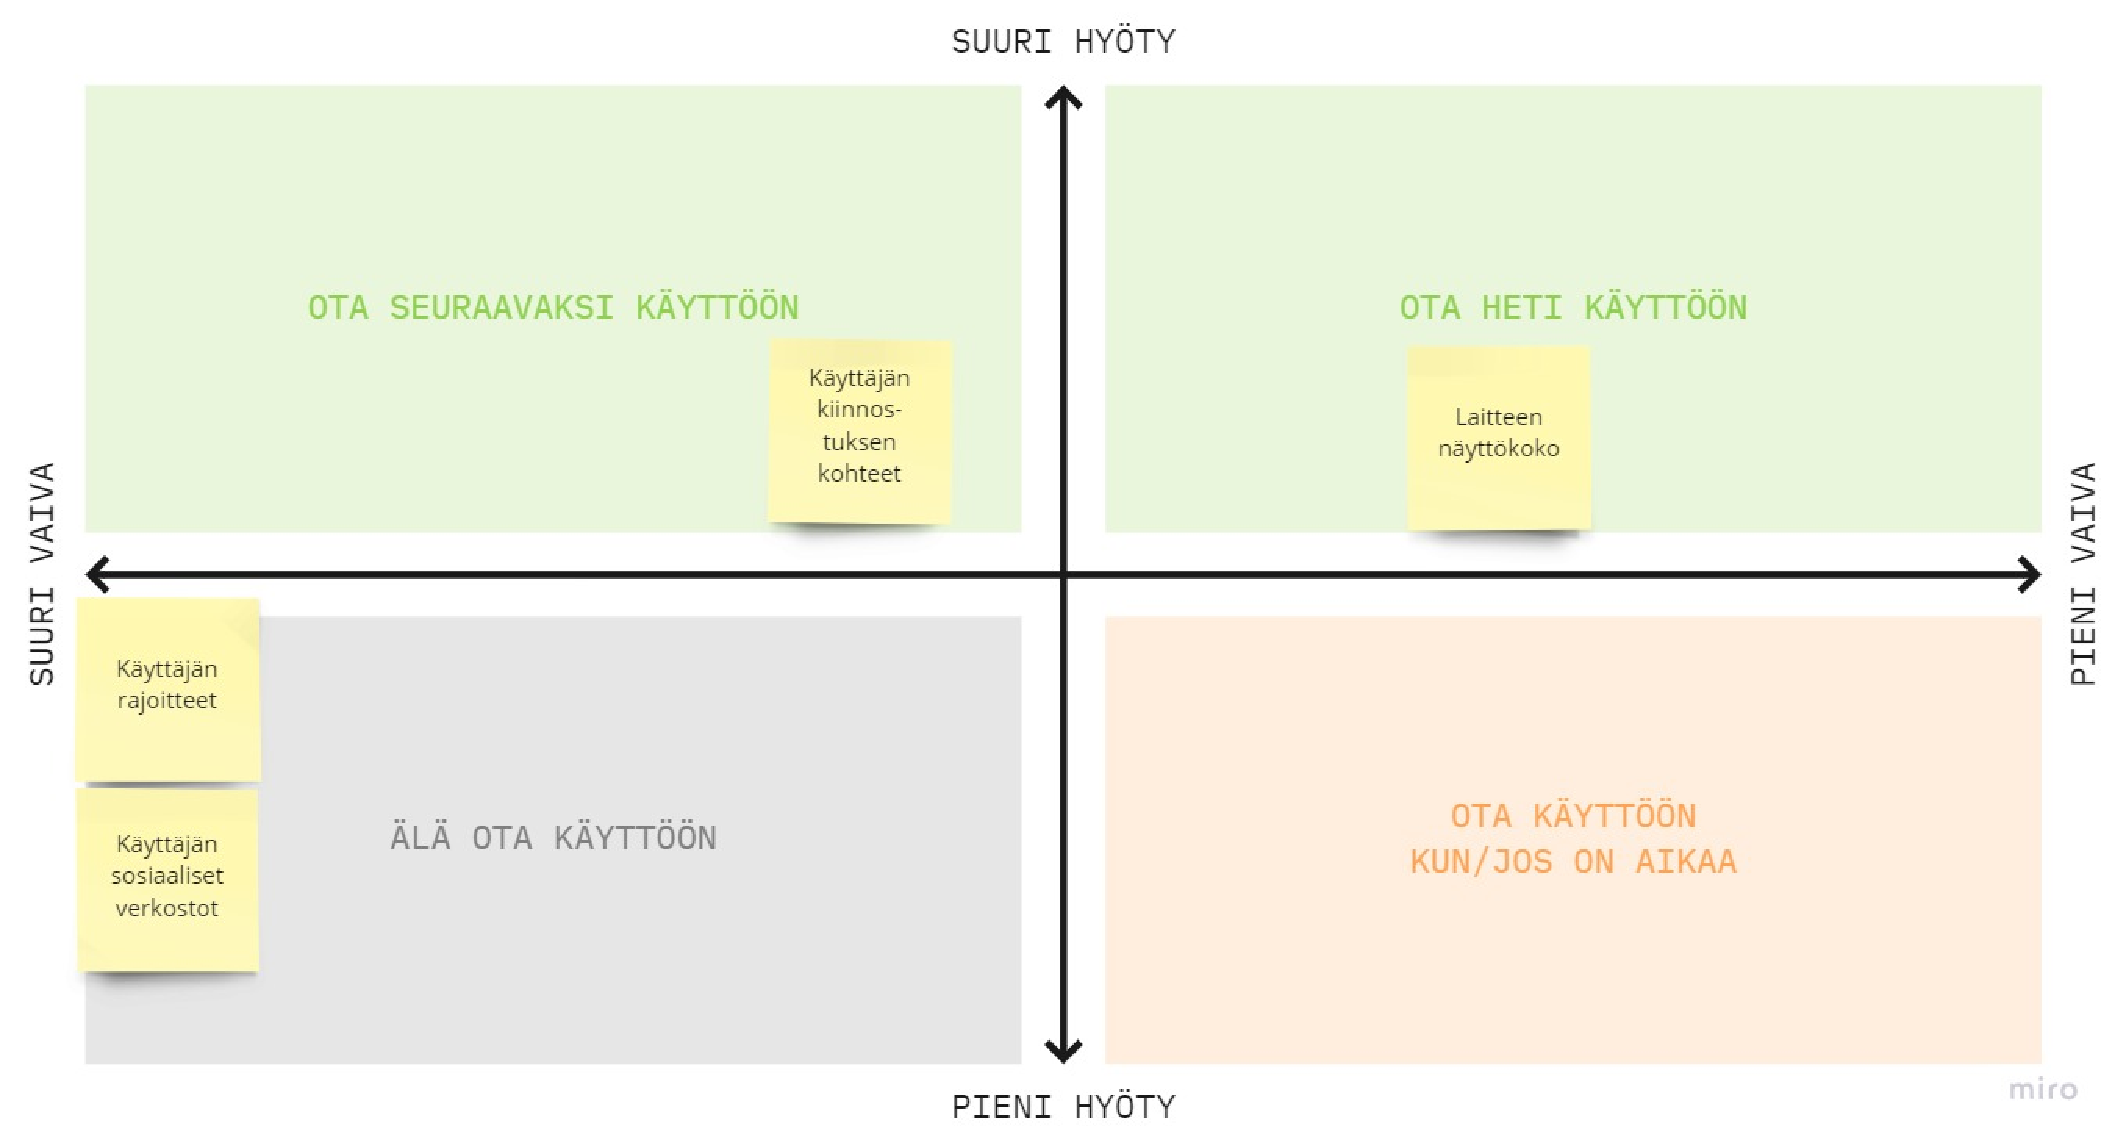
\includegraphics[width=\textwidth]{images/layout-priorization.pdf}
    \caption{Tärkeimmät sisällön asettelun personointimenetelmät.~\label{fig:layout-priorization}}
\end{figure}

\subsubsection{Typografia}

{\tiny\tabcolsep=3pt
    \begin{longtable}{p{2.5cm}|p{6cm}|p{0.5cm}p{0.5cm}p{0.5cm}|p{0.5cm}|p{0.5cm}p{0.5cm}p{0.5cm}|p{0.5cm}|}
        \multirow[t]{2}{*}{\textbf{Näkökulma}} & \multirow[t]{2}{*}{\textbf{Menetelmän kuvaus}}                                                                                                                                                                                                                & \multicolumn{4}{c|}{\textbf{Vaivattomuus}} & \multicolumn{4}{c|}{\textbf{Hyöty}}                                                                                                                                                                                                                                                  \\\cline{3-10}
                                               &                                                                                                                                                                                                                                                               & \vertical{\textbf{Toteutuksen helppous}}   & \vertical{\textbf{Monistettavuus}}  & \vertical{\textbf{Käyttö toimialalla}} & \vertical{\textbf{Yhteensä}} & \vertical{\textbf{Vaikutus käyttökokemukseen}~} & \vertical{\textbf{Kohdennuksen tarkkuus}} & \vertical{\textbf{Tulevaisuuden näkymät}} & \vertical{\textbf{Yhteensä}} \\
        \midrule
        \textbf{Käyttäjä}                                                                                                                                                                                                                                                                                                                                                                                                                                                                                                                                                                                                                          \\
        \midrule
        Rajoitteet                             & Rello ym.~\cite{10.1145/2207016.2207048} tutkivat web-typografian personointia lukihäiriön näkökulmasta. Hyöty typografian personoinnista lukihäiriöstä kärsiville on merkittävä. Tieto rajoitteista kerättävä käyttäjältä erikseen.                          & 1                                          & 0                                   & 0                                      & 1                            & 10                                              & 1                                         & 1                                         & 12                           \\
        \midrule
        Ikä                                    & Hussain ym.~\cite{hussain_sohaib_ahmed_qasim_khan_2011} löysivät eroja eri ikäryhmien typografiamieltymyksissä. Käytännön hyöty on vielä epäselvä.                                                                                                            & 1                                          & 1                                   & 0                                      & 2                            & 1                                               & 1                                         & 0                                         & 2                            \\
        \midrule
        Sukupuoli                              & Vaikutusta ei ole tutkittu.                                                                                                                                                                                                                                   & 0                                          & 1                                   & 0                                      & 1                            & 0                                               & 0                                         & 0                                         & 0                            \\
        \midrule
        Kulttuuritausta                        & Reinecke ym.~\cite{10.1145/2556288.2557052} eivät ota tutkimuksessaan suoraan kantaa typografian personoinnin hyötyihin, joten vaikutusta ei ole tutkittu. Eri kirjoitusjärjestelmät täytyy ottaa huomioon sisällön näkökulmasta.                             & 0                                          & 1                                   & 0                                      & 1                            & 0                                               & 1                                         & 0                                         & 1                            \\
        \midrule
        Koulutustausta                         & Vaikutusta ei ole tutkittu. Tieto koulutustaustasta saatavilla julkishallinnon tietokannoista tai käyttäjältä erikseen pyydettynä.                                                                                                                            & 0                                          & 0                                   & 0                                      & 0                            & 0                                               & 1                                         & 0                                         & 1                            \\
        \midrule
        Kiinnostuksen kohteet                  & Vaikutusta ei ole tutkittu. Kiinnostuksen kohteet pääteltävissä käyttäytymisestä sivustolla.                                                                                                                                                                  & 0                                          & 1                                   & 0                                      & 1                            & 0                                               & 10                                        & 0                                         & 10                           \\
        \midrule
        Mieliala                               & Choi ja Aizawa~\cite{choi_aizawa_2018} löysivät, että typografian muuttaminen mielialan mukaan tekee viestittelystä eläväisempää. Ei selkeää keinoa kerätä tietoa.                                                                                            & 1                                          & 0                                   & 0                                      & 1                            & 10                                              & 1                                         & 0                                         & 11                           \\
        \midrule
        Sosiaaliset verkostot                  & Vaikutusta ei ole tutkittu. Tieto saatavilla suuntaa-antavasti sosiaalisen median kautta käyttäjän suostumuksella.                                                                                                                                            & 0                                          & 0                                   & 0                                      & 0                            & 0                                               & 10                                        & 0                                         & 10                           \\
        \midrule
        \textbf{Käyttöympäristö}                                                                                                                                                                                                                                                                                                                                                                                                                                                                                                                                                                                                                   \\
        \midrule
        Laitteen näyttökoko                    & Darroch ym.~\cite{10.1007/11555261_23} löysivät yhteyden laitteen näyttökoon ja kirjasinkoon välillä. Kirjasinkoko mobiililaitteilla huomioidaan osana responsiivista web-suunnittelua.                                                                       & 10                                         & 0                                   & 10                                     & 20                           & 10                                              & 0                                         & 1                                         & 11                           \\
        \midrule
        Laitteen suorituskyky                  & Vaikutusta ei ole tutkittu.                                                                                                                                                                                                                                   & 0                                          & 1                                   & 0                                      & 1                            & 0                                               & 0                                         & 0                                         & 0                            \\
        \midrule
        Verkkoyhteyden laatu                   & Vaikutusta ei ole tutkittu, mutta hyöty on ilmeinen. Viime vuosina toimialalla on kehitetty ratkaisuja kuten esilataus~\cite{grigorik_2020} kirjasintyyppien latausajan minimoiseksi.                                                                         & 10                                         & 10                                  & 10                                     & 30                           & 10                                              & 0                                         & 10                                        & 20                           \\
        \midrule
        Sijainti                               & Vaikutusta ei ole tutkittu. Tieto saatavilla selainrajapintojen kautta käyttäjän suostumuksella.                                                                                                                                                              & 0                                          & 1                                   & 0                                      & 1                            & 0                                               & 1                                         & 0                                         & 1                            \\
        \midrule
        Aika                                   & Vaikutusta ei ole tutkittu.                                                                                                                                                                                                                                   & 0                                          & 1                                   & 0                                      & 1                            & 0                                               & 0                                         & 0                                         & 0                            \\
        \midrule
        Kirkkaus                               & Vaikutusta ei ole tutkittu, mutta hyöty vaikuttaa selkeältä. Tekstin kontrastin parantaminen kirkkaassa auringonvalossa esimerkiksi kirjasinkokoa suurentamalla on selkeä sovelluskohde. Tieto saatavilla selainrajapintojen kautta käyttäjän suostumuksella. & 0                                          & 1                                   & 0                                      & 1                            & 10                                              & 1                                         & 0                                         & 11                           \\
        \midrule
        Äänekkyys                              & Vaikutusta ei ole tutkittu. Tieto saatavilla selainrajapintojen kautta käyttäjän suostumuksella.                                                                                                                                                              & 0                                          & 1                                   & 0                                      & 1                            & 0                                               & 0                                         & 0                                         & 0                            \\
        \midrule
        Lämpötila ja sää                       & Vaikutusta ei ole tutkittu. Käyttäjän suostumuksella sijaintietoa voidaan käyttää säätietojen hakemiseen kolmannen osapuolen rajapinnasta.                                                                                                                    & 0                                          & 1                                   & 0                                      & 1                            & 0                                               & 0                                         & 0                                         & 0                            \\
        \midrule
        Liike                                  & Vaikutusta ei ole tutkittu, mutta ympäristön kirkkauden tapaan myös liikkeen tapauksessa tekstin kontrastin kasvattaminen parantaa luettavuutta. Tieto saatavilla selainrajapintojen kautta käyttäjän suostumuksella.                                         & 0                                          & 1                                   & 0                                      & 1                            & 10                                              & 1                                         & 0                                         & 11                           \\
    \end{longtable}
}

Typografian personointimenetelmien vertailussa korostuu sisällön asettelun
tapaan responsiivinen web-suunnittelu. Tekstin tulee olla luettavaa kaikilla
laitteilla, ja siksi esimerkiksi kirjasinkoon suurentaminen mobiililaitteilla on
erittäin hyödyllistä. Lisäksi tekstin luettavuuteen vaikuttavat tekijät kuten
ympäristön kirkkaus ja laitteen liike, kuten tärinä nousevat hyödyllisiksi. Ne
eivät kuitenkaan tällä hetkellä ole helposti personoitavissa. Käyttäjälle
personoitava typografia ei nouse vertailussa kovin hyödylliseksi, vaan
tärkeimmät menetelmät painottuvat käyttöympäristön näkökulmien puolelle.
Tärkeimmät typografian personointimenetelmät on merkitty
kuvaan~\ref{fig:typography-priorization}.

\begin{figure}[htb]
    \centering
    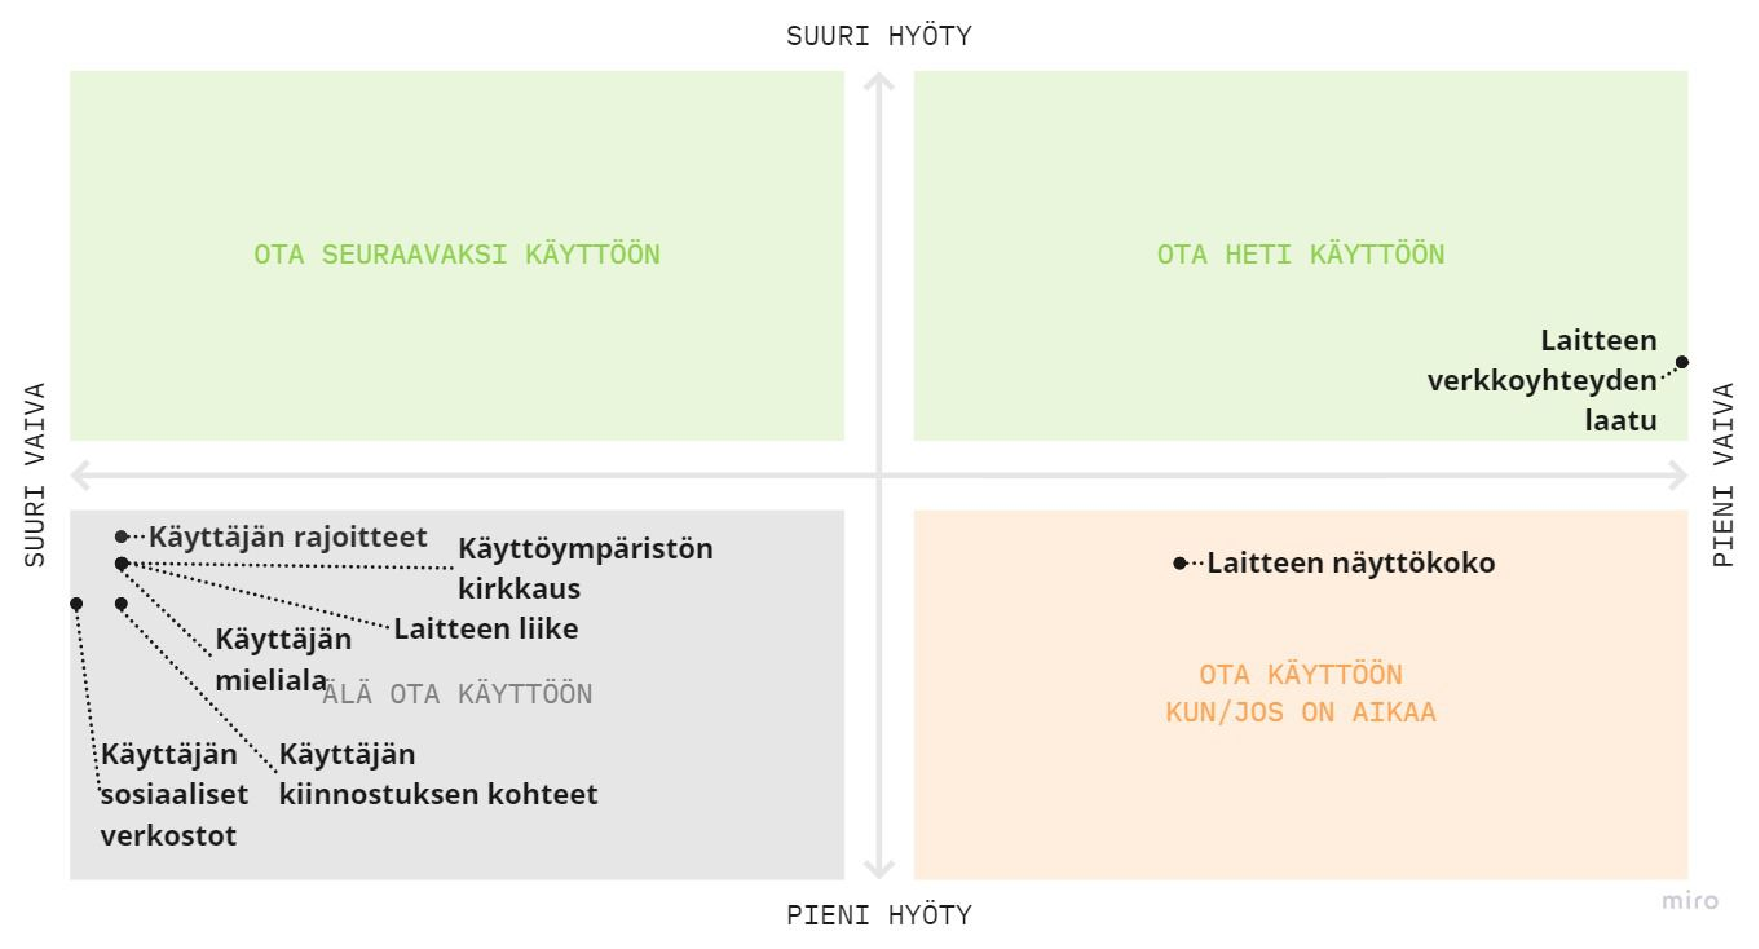
\includegraphics[width=\textwidth]{images/typography-priorization.pdf}
    \caption{Tärkeimmät typografian personointimenetelmät.~\label{fig:typography-priorization}}
\end{figure}

\subsubsection{Värit}

{\tiny\tabcolsep=3pt
    \begin{longtable}{p{2.5cm}|p{6cm}|p{0.5cm}p{0.5cm}p{0.5cm}|p{0.5cm}|p{0.5cm}p{0.5cm}p{0.5cm}|p{0.5cm}|}
        \multirow[t]{2}{*}{\textbf{Näkökulma}} & \multirow[t]{2}{*}{\textbf{Menetelmän kuvaus}}                                                                                                                                                                                                                                                                           & \multicolumn{4}{c|}{\textbf{Vaivattomuus}} & \multicolumn{4}{c|}{\textbf{Hyöty}}                                                                                                                                                                                                                                                  \\\cline{3-10}
                                               &                                                                                                                                                                                                                                                                                                                          & \vertical{\textbf{Toteutuksen helppous}}   & \vertical{\textbf{Monistettavuus}}  & \vertical{\textbf{Käyttö toimialalla}} & \vertical{\textbf{Yhteensä}} & \vertical{\textbf{Vaikutus käyttökokemukseen}~} & \vertical{\textbf{Kohdennuksen tarkkuus}} & \vertical{\textbf{Tulevaisuuden näkymät}} & \vertical{\textbf{Yhteensä}} \\
        \midrule
        \textbf{Käyttäjä}                                                                                                                                                                                                                                                                                                                                                                                                                                                                                                                                                                                                                                                                                     \\
        \midrule
        Rajoitteet                             & Väripaletin personointi värisokeille kävijöille olisi hyödyllistä varsinkin graafisten sisältöjen ymmärtämisessä. Jefferson ja Harvey kehittivät menetelmän, jolla web-sivuston väripaletin voi automaattisesti korjata värisokeille.~\cite{10.1145/1168987.1168996}. Tieto rajoitteista kerättävä käyttäjältä erikseen. & 1                                          & 0                                   & 0                                      & 1                            & 10                                              & 1                                         & 1                                         & 12                           \\
        \midrule
        Ikä                                    & Reinecke ym.~\cite{10.1145/2556288.2557052} löysivät, että ikä vaikuttaa miellyttäväksi koettuihin väreihin. Käytännön hyöty on vielä epäselvä.                                                                                                                                                                          & 1                                          & 1                                   & 0                                      & 2                            & 1                                               & 1                                         & 0                                         & 2                            \\
        \midrule
        Sukupuoli                              & Reinecke ym.~\cite{10.1145/2556288.2557052} löysivät, että sukupuoli vaikuttaa miellyttäväksi koettuihin väreihin. Käytännön hyöty on vielä epäselvä.                                                                                                                                                                    & 1                                          & 1                                   & 0                                      & 2                            & 1                                               & 1                                         & 0                                         & 2                            \\
        \midrule
        Kulttuuritausta                        & Reinecke ym.~\cite{10.1145/2556288.2557052} löysivät, että kulttuuritausta vaikuttaa miellyttäväksi koettuihin väreihin. Käytännön hyöty on vielä epäselvä.                                                                                                                                                              & 1                                          & 1                                   & 0                                      & 2                            & 1                                               & 1                                         & 0                                         & 2                            \\
        \midrule
        Koulutustausta                         & Vaikutusta ei ole tutkittu. Tieto koulutustaustasta saatavilla julkishallinnon tietokannoista tai käyttäjältä erikseen pyydettynä.                                                                                                                                                                                       & 0                                          & 1                                   & 0                                      & 1                            & 0                                               & 1                                         & 0                                         & 1                            \\
        \midrule
        Kiinnostuksen kohteet                  & Vaikutusta ei ole tutkittu, mutta Salesforcen Einstein Designer -konsepti personoi myös värejä sivustokäyttäytymisen pohjalta.                                                                                                                                                                                           & 0                                          & 10                                  & 1                                      & 11                           & 1                                               & 10                                        & 10                                        & 21                           \\
        \midrule
        Mieliala                               & Vaikutusta ei ole tutkittu. Ei selkeää keinoa kerätä tietoa.                                                                                                                                                                                                                                                             & 0                                          & 0                                   & 0                                      & 0                            & 1                                               & 1                                         & 0                                         & 2                            \\
        \midrule
        Sosiaaliset verkostot                  & Vaikutusta ei ole tutkittu. Tieto saatavilla suuntaa-antavasti sosiaalisen median kautta käyttäjän suostumuksella.                                                                                                                                                                                                       & 0                                          & 0                                   & 0                                      & 0                            & 0                                               & 10                                        & 0                                         & 10                           \\
        \midrule
        \textbf{Käyttöympäristö}                                                                                                                                                                                                                                                                                                                                                                                                                                                                                                                                                                                                                                                                              \\
        \midrule
        Laitteen näyttökoko                    & Vaikutusta ei ole tutkittu.                                                                                                                                                                                                                                                                                              & 0                                          & 1                                   & 0                                      & 1                            & 0                                               & 0                                         & 0                                         & 0                            \\
        \midrule
        Laitteen suorituskyky                  & Vaikutusta ei ole tutkittu.                                                                                                                                                                                                                                                                                              & 0                                          & 1                                   & 0                                      & 1                            & 0                                               & 0                                         & 0                                         & 0                            \\
        \midrule
        Verkkoyhteyden laatu                   & Vaikutusta ei ole tutkittu.                                                                                                                                                                                                                                                                                              & 0                                          & 1                                   & 0                                      & 1                            & 0                                               & 0                                         & 0                                         & 0                            \\
        \midrule
        Sijainti                               & Vaikutusta ei ole tutkittu. Tieto saatavilla selainrajapintojen kautta käyttäjän suostumuksella.                                                                                                                                                                                                                         & 0                                          & 1                                   & 0                                      & 1                            & 0                                               & 0                                         & 0                                         & 0                            \\
        \midrule
        Aika                                   & Vaikutusta ei ole tutkittu.                                                                                                                                                                                                                                                                                              & 0                                          & 1                                   & 0                                      & 1                            & 0                                               & 0                                         & 0                                         & 0                            \\
        \midrule
        Kirkkaus                               & Vaikutusta ei ole tutkittu, mutta hyöty vaikuttaa typografian tapaan selkeältä, joskaan ei yhtä merkittävältä värien toissijaisuuden vuoksi.                                                                                                                                                                             & 0                                          & 1                                   & 0                                      & 1                            & 1                                               & 1                                         & 0                                         & 2                            \\
        \midrule
        Äänekkyys                              & Vaikutusta ei ole tutkittu. Tieto saatavilla selainrajapintojen kautta käyttäjän suostumuksella.                                                                                                                                                                                                                         & 0                                          & 1                                   & 0                                      & 1                            & 0                                               & 0                                         & 0                                         & 0                            \\
        \midrule
        Lämpötila ja sää                       & Vaikutusta ei ole tutkittu. Käyttäjän suostumuksella sijaintietoa voidaan käyttää säätietojen hakemiseen kolmannen osapuolen rajapinnasta.                                                                                                                                                                               & 0                                          & 1                                   & 0                                      & 1                            & 0                                               & 0                                         & 0                                         & 0                            \\
        \midrule
        Liike                                  & Vaikutusta ei ole tutkittu. Tieto saatavilla selainrajapintojen kautta käyttäjän suostumuksella.                                                                                                                                                                                                                         & 0                                          & 1                                   & 0                                      & 1                            & 0                                               & 0                                         & 0                                         & 0                            \\
    \end{longtable}
}

Värien personoinnissa ei nouse esiin merkittävän hyödyllisiä
personointikohteita. Reinecke ym.~\cite{10.1145/2556288.2557052} tutkimus kyllä
osoittaa yhteyden värimieltymysten ja erinäisten ominaisuuksien, kuten iän ja
sukupuolen välillä, mutta käytännön tasolla menetelmät on hankala ottaa käyttöön
web-sivustolla. Värien osalta tärkeimmät personointimenetelmät ovat värisokeuden
huomioiminen ja käyttäjän kiinnostuksen kohteiden pohjalta tehtävä ulkoasun
personointi, jota muun muassa Salesforcen Einstein Designer -konsepti on
demonstroinut. Tärkeimmät värien personointimenetelmät on merkitty
kuvaan~\ref{fig:color-priorization}.

\begin{figure}[htb]
    \centering
    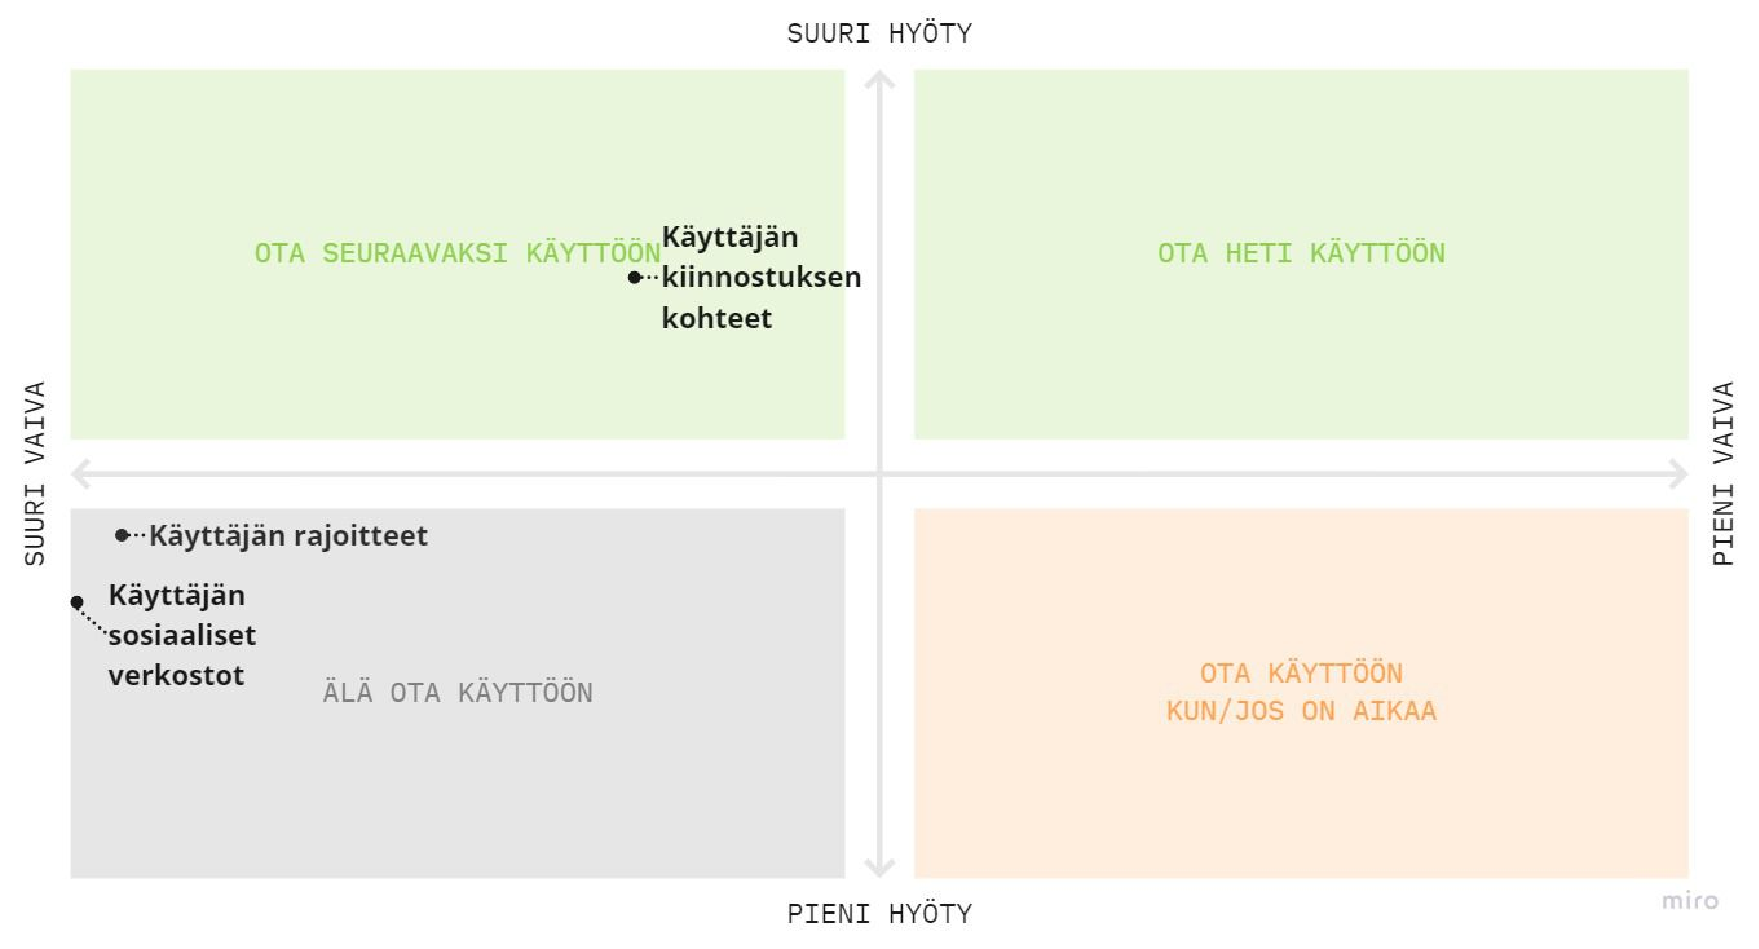
\includegraphics[width=\textwidth]{images/color-priorization.pdf}
    \caption{Tärkeimmät värien personointimenetelmät.~\label{fig:color-priorization}}
\end{figure}

\subsubsection{Kuvien muokkaus}

{\tiny\tabcolsep=3pt
    \begin{longtable}{p{2.5cm}|p{6cm}|p{0.5cm}p{0.5cm}p{0.5cm}|p{0.5cm}|p{0.5cm}p{0.5cm}p{0.5cm}|p{0.5cm}|}
        \multirow[t]{2}{*}{\textbf{Näkökulma}} & \multirow[t]{2}{*}{\textbf{Menetelmän kuvaus}}                                                                                                                                                                                                                                                                                                                            & \multicolumn{4}{c|}{\textbf{Vaivattomuus}} & \multicolumn{4}{c|}{\textbf{Hyöty}}                                                                                                                                                                                                                                                  \\\cline{3-10}
                                               &                                                                                                                                                                                                                                                                                                                                                                           & \vertical{\textbf{Toteutuksen helppous}}   & \vertical{\textbf{Monistettavuus}}  & \vertical{\textbf{Käyttö toimialalla}} & \vertical{\textbf{Yhteensä}} & \vertical{\textbf{Vaikutus käyttökokemukseen}~} & \vertical{\textbf{Kohdennuksen tarkkuus}} & \vertical{\textbf{Tulevaisuuden näkymät}} & \vertical{\textbf{Yhteensä}} \\
        \midrule
        \textbf{Käyttäjä}                                                                                                                                                                                                                                                                                                                                                                                                                                                                                                                                                                                                                                                                                                                                      \\
        \midrule
        Rajoitteet                             & Vaikutusta ei ole suoraan tutkittu, mutta hyödyt samansuuntaisia kuin Jeffersonin ja Harveyn tutkimuksessa~\cite{10.1145/1168987.1168996}, jossa tarkasteltiin värien optimointia värisokeille. Hyödyt eivät ole yhtä merkittäviä, koska kuvia ei voida samaan tapaan vapaasti muokata kuin web-sivuston väripalettia. Tieto rajoitteista kerättävä käyttäjältä erikseen. & 0                                          & 0                                   & 0                                      & 0                            & 1                                               & 1                                         & 0                                         & 2                            \\
        \midrule
        Ikä                                    & Vaikutusta ei ole suoraan tutkittu, mutta kuvien kontrastin kasvattamisesta voisi olla hyötyä ikääntyneille.                                                                                                                                                                                                                                                              & 0                                          & 1                                   & 0                                      & 1                            & 1                                               & 1                                         & 0                                         & 2                            \\
        \midrule
        Sukupuoli                              & Vaikutusta ei ole tutkittu.                                                                                                                                                                                                                                                                                                                                               & 0                                          & 1                                   & 0                                      & 1                            & 0                                               & 1                                         & 0                                         & 1                            \\
        \midrule
        Kulttuuritausta                        & Vaikutusta ei ole tutkittu.                                                                                                                                                                                                                                                                                                                                               & 0                                          & 0                                   & 0                                      & 0                            & 0                                               & 1                                         & 0                                         & 1                            \\
        \midrule
        Koulutustausta                         & Vaikutusta ei ole tutkittu. Tieto koulutustaustasta saatavilla julkishallinnon tietokannoista tai käyttäjältä erikseen pyydettynä.                                                                                                                                                                                                                                        & 0                                          & 0                                   & 0                                      & 0                            & 0                                               & 1                                         & 0                                         & 1                            \\
        \midrule
        Kiinnostuksen kohteet                  & Kang ym.~\cite{5539850} löysivät, että käyttäjä suosii omien mieltymystensä mukaan muokattuja kuvia. Kim ym.~\cite{10.1007/978-3-030-58577-8_23} jatkokehittivät Kang ym.~menetelmää ja julkaisivat referenssitoteutuksensa. Mieltymykset täytyy kerätä erikseen käyttäjältä etukäteen.                                                                                   & 10                                         & 0                                   & 0                                      & 10                           & 10                                              & 10                                        & 1                                         & 21                           \\
        \midrule
        Mieliala                               & Vaikutusta ei ole tutkittu, mutta Kang ym.\cite{5539850} tulokset pätevät jos käyttäjän mieltymykset kerätään halutussa mielialassa.                                                                                                                                                                                                                                      & 0                                          & 0                                   & 0                                      & 0                            & 10                                              & 10                                        & 0                                         & 20                           \\
        \midrule
        Sosiaaliset verkostot                  & Vaikutusta ei ole tutkittu. Tieto saatavilla suuntaa-antavasti sosiaalisen median kautta käyttäjän suostumuksella.                                                                                                                                                                                                                                                        & 0                                          & 0                                   & 0                                      & 0                            & 0                                               & 10                                        & 0                                         & 10                           \\
        \midrule
        \textbf{Käyttöympäristö}                                                                                                                                                                                                                                                                                                                                                                                                                                                                                                                                                                                                                                                                                                                               \\
        \midrule
        Laitteen näyttökoko                    & Kuvien älykäs rajaus eri näyttöko'oille on hyödyllistä. Kang ym.~\cite{5539850} pohtivat että tutkimusta ja vaikutusten arviointia voisi jatkaa myös rajauksen optimoinnin osalta, mutta tällä haavaa vaikutusta ei ole vielä tutkittu. Toimialalla on useita ratkaisuja älykkääseen rajaukseen (engl.~\textit{smart cropping}).                                          & 10                                         & 10                                  & 10                                     & 30                           & 10                                              & 1                                         & 10                                        & 21                           \\
        \midrule
        Laitteen suorituskyky                  & Vaikutusta ei ole tutkittu.                                                                                                                                                                                                                                                                                                                                               & 0                                          & 0                                   & 0                                      & 0                            & 0                                               & 0                                         & 0                                         & 0                            \\
        \midrule
        Verkkoyhteyden laatu                   & Vaikutusta ei ole tutkittu, mutta viime vuosina on kehitetty useita kuvaformaatteja, kuten WebP ja AVIF, jotka pakkaavat kuvan tehokkaamin kuin perinteiset JPEG tai PNG, ja vievät siten vähemmän tilaa. Kuvaformaatin personointi verkkoyhteyden laadun perusteella tuo siis merkittäviä hyötyjä.                                                                       & 10                                         & 10                                  & 10                                     & 30                           & 10                                              & 0                                         & 10                                        & 20                           \\
        \midrule
        Sijainti                               & Vaikutusta ei ole tutkittu. Tieto saatavilla selainrajapintojen kautta käyttäjän suostumuksella.                                                                                                                                                                                                                                                                          & 0                                          & 1                                   & 0                                      & 1                            & 0                                               & 0                                         & 0                                         & 0                            \\
        \midrule
        Aika                                   & Vaikutusta ei ole tutkittu.                                                                                                                                                                                                                                                                                                                                               & 0                                          & 1                                   & 0                                      & 1                            & 0                                               & 0                                         & 0                                         & 0                            \\
        \midrule
        Kirkkaus                               & Vaikutusta ei ole tutkittu, mutta hyöty vaikuttaa typografian tapaan selkeältä. Kirkkaassa auringonpaisteessa kuvan kontrastia voidaan kasvattaa. Pimeässä kuva voidaan esittää yötilan kaltaisesti.                                                                                                                                                                      & 0                                          & 1                                   & 0                                      & 1                            & 10                                              & 1                                         & 0                                         & 11                           \\
        \midrule
        Äänekkyys                              & Vaikutusta ei ole tutkittu. Tieto saatavilla selainrajapintojen kautta käyttäjän suostumuksella.                                                                                                                                                                                                                                                                          & 0                                          & 1                                   & 0                                      & 1                            & 0                                               & 0                                         & 0                                         & 0                            \\
        \midrule
        Lämpötila ja sää                       & Vaikutusta ei ole tutkittu. Tieto saatavilla selainrajapintojen kautta käyttäjän suostumuksella.                                                                                                                                                                                                                                                                          & 0                                          & 1                                   & 0                                      & 1                            & 0                                               & 0                                         & 0                                         & 0                            \\
        \midrule
        Liike                                  & Vaikutusta ei ole tutkittu. Tieto saatavilla selainrajapintojen kautta käyttäjän suostumuksella.                                                                                                                                                                                                                                                                          & 0                                          & 1                                   & 0                                      & 1                            & 0                                               & 0                                         & 0                                         & 0                            \\
    \end{longtable}
}

Kuvien muokkaus nousee personointinäkökulmien ja -menetelmien vertailussa
sisällön asettelun rinnalle arvioidussa tärkeydessä. Kuvien muokkauksen
personoinnissa korostuu sisällön asettelun tapaan responsiivinen
web-suunnittelu, eli esimerkiksi kuvaformaattien optimointi heikolle
verkkoyhteydelle ja kuvien älykäs rajaus mobiililaitteille. Myös käyttäjän
rajoitusten, kuten huonon näön tai värisokeuden huomioinen nousee tärkeäksi
personointikeinoksi. Myös Kang ym.~\cite{5539850} tutkimuksessa kuvattu
käyttäjän mieltymysten mukainen kuvien muokkaus vaikuttaa lupaavalta. Tärkeimmät
Värien personointimenetelmät on merkitty kuvaan~\ref{fig:images-priorization}.

\begin{figure}[htb]
    \centering
    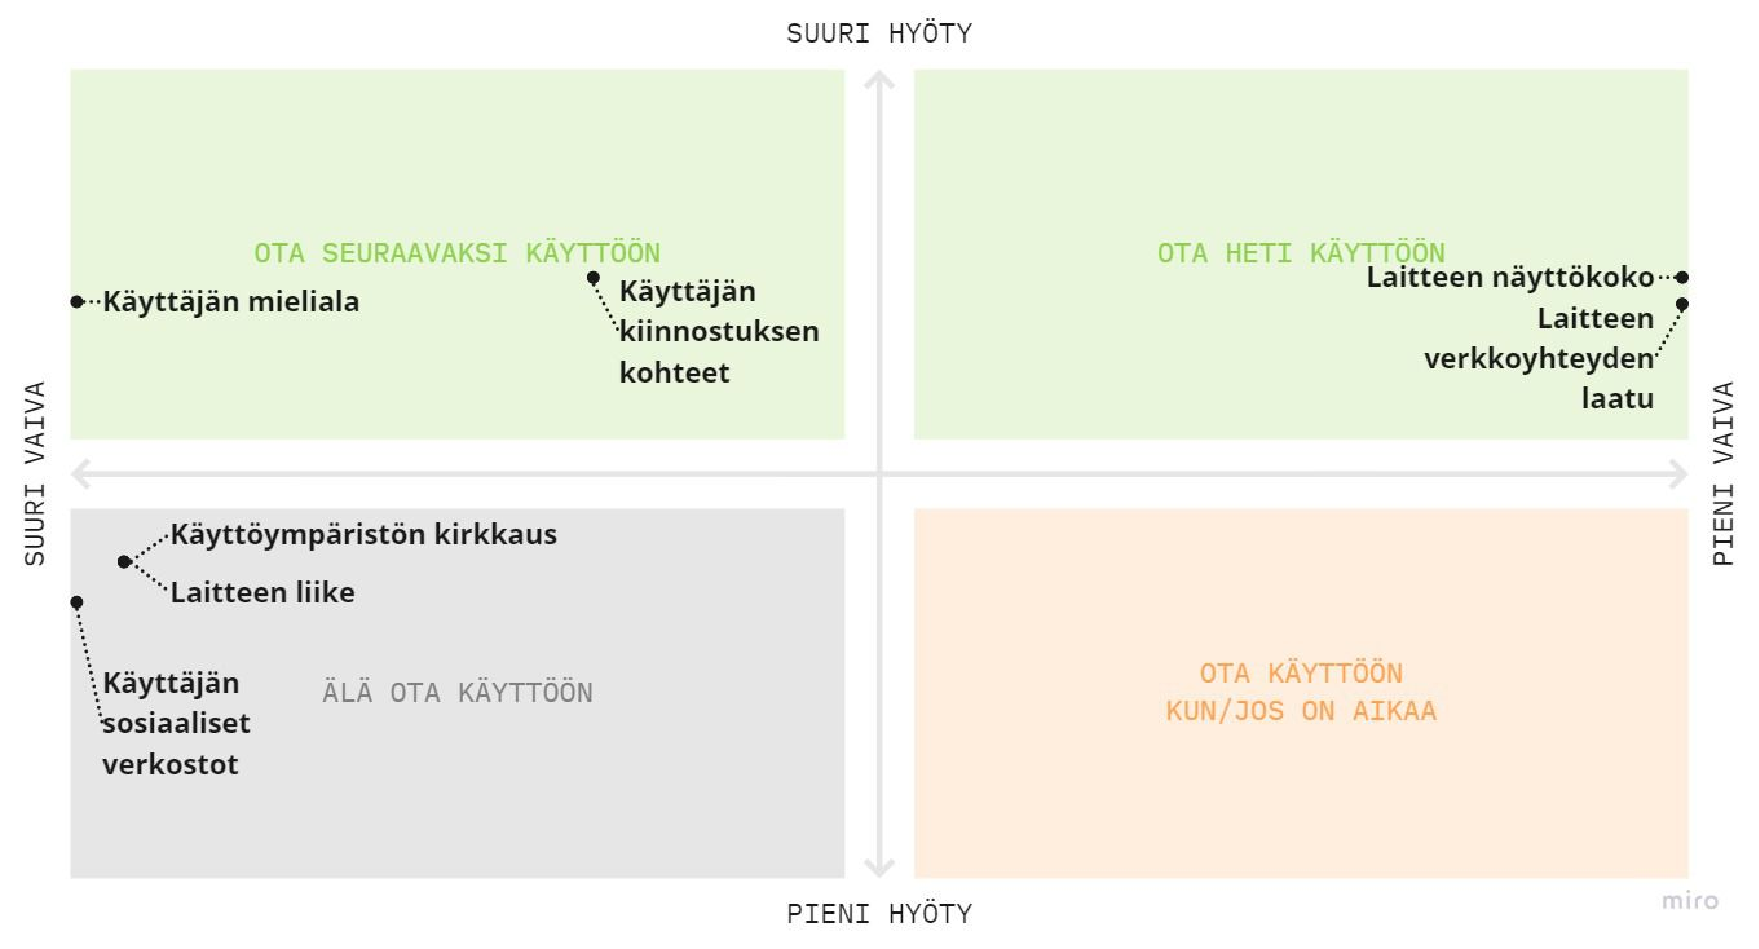
\includegraphics[width=\textwidth]{images/images-priorization.pdf}
    \caption{Tärkeimmät kuvien muokkauksen personointimenetelmät.~\label{fig:images-priorization}}
\end{figure}

\subsection{Yhteenveto}

Tähän yhteinen kuva kaikista menetelmistä.

\clearpage

\section{Yhteenveto}

\clearpage

\thesisbibliography{}
\printbibliography{}

\end{document}
